\chapter{Ejercicio de cronometraje de vueltas competitivas con Gazebo y ROS}\label{cap.chrono}
En este capítulo del TFG ya se han definido el contexto, los objetivos y las herramientas utilizadas para la consecución de este proyecto. En este capítulo abordaremos todo lo relacionado con el desarrollo de una de las prácticas llamada \textit{Chrono}. Esta práctica forma parte del conjunto de prácticas de \textit{JdeRobot}. Se explicará la infraestructura de soporte de la práctica, el software y el funcionamiento de la práctica.

\section{Enunciado}\label{sec.enunciado}
El objetivo de esta práctica, enfocado al estudiante, es el desarrollo de un algoritmo que dote de la inteligencia necesaria a un modelo de robot F1 que compite con el récord grabado para el circuito. De esta manera, no solo se permite el desarrollo de un algoritmo funcional, sino que se propone un avance en el grado de dificultad exigiendo al alumno que optimice su algoritmo para que consiga completar una vuelta al circuito sin colisionar y con un tiempo inferior al ofrecido.

Para desarrollar la solución del algoritmo, el alumno deberá abordar distintos problemas relacionados con la programación. El primero de ellos es programar un algoritmo para realizar un filtrado de la imagen que capta el robot F1 por su cámara y escoger la línea roja central del circuito. Tras esto, el alumno deberá desarrollar un algoritmo que establezca un avance controlado del robot F1 para que siga la línea roja que ha sido filtrada por el algoritmo anterior.

Como puede observarse en los problemas abordados, además de tener que afrontar los problemas, es necesario que sean abordados conjuntamente, ya que el movimiento controlado del modelo depende del filtrado de las imágenes. Para añadir dificultad a la práctica, es necesario que el algoritmo de control de movimiento del vehículo sea eficaz dado que, de otro modo, será más lento que la solución proporcionada y llegará en segundo lugar.

\section{Infraestructura}
En esta sección se abordarán los distintos elementos involucrados en la práctica (Figura \ref{fig.infraestructura_ch}).

\begin{figure}[H]
  \begin{center}
    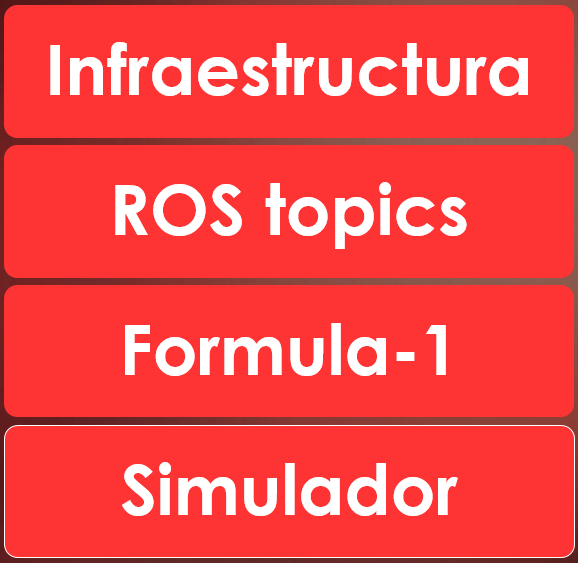
\includegraphics[width=0.4\linewidth, height=8cm]{figures/infraestructura_ch.png}
		\caption{Infraestructura de Chrono}
		\label{fig.infraestructura_ch}
		\end{center}
\end{figure}

\subsection{Modelo de robot F1}
El robot que se ha utilizado para esta práctica es un modelo de robot terrestre móvil que cuenta con 4 ruedas. El chasis elegido corresponde a un modelo de F1, específicamente del modelo RedBull. Además de este modelo se han incluido un gran conjunto de modelos de F1 correspondientes a las principales escuderías que participan en la Fórmula 1. Esto supone un total de 12 modelos de coches de escuderías reales (India, HRT, Lotus, Mclaren, Mercedes, RedBull, Renault, Tororroso, Virgin y Williams) y un modelos sin marca comercial. Además, para cada modelo de coche ha sido necesario el desarrollo de dos modelos distintos, uno que incorpora una cámara, para esta práctica, y otro modelo que tiene un láser para otras prácticas de \textit{JdeRobot}. Gracias a estos modelos, en la práctica actual puede usarse indistintamente el modelo preferido por el estudiante (Figura \ref{fig.f1s}).

\begin{figure}[H]
  \begin{center}
    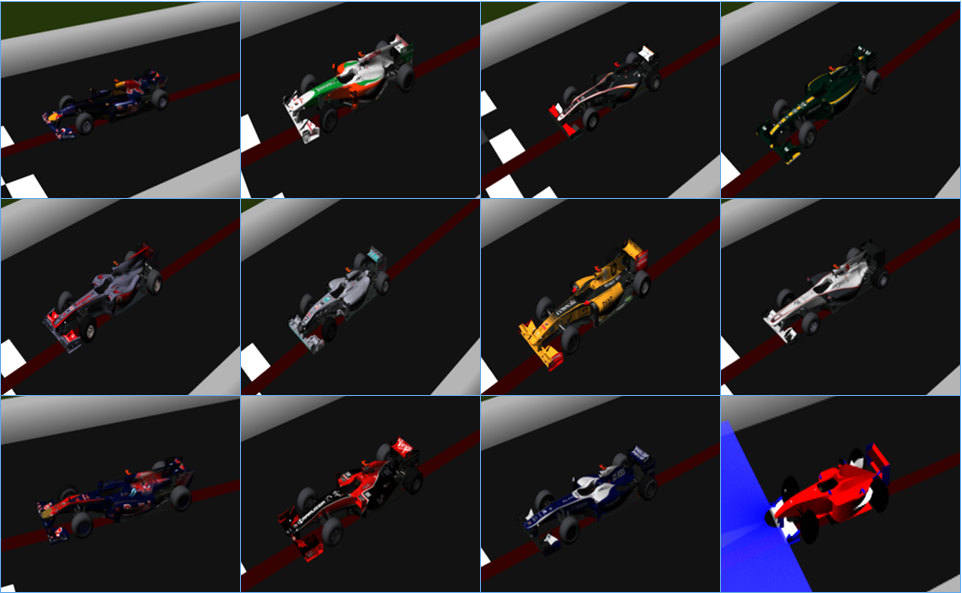
\includegraphics[width=0.99\linewidth, height=5.5cm]{figures/coches.png}
		\caption{Modelos disponibles de coches}
		\label{fig.f1s}
		\end{center}
\end{figure}

Cualquiera de los modelos de la Figura \ref{fig.f1s} utiliza los \textit{plugins} de ROS para dotar al modelo de movimiento, captación de imágenes y odometría. Estos \textit{plugins} son ofrecidos por las librerías de \textit{ROS Kinetic}:

\begin{itemize}
	\item \textit{libgazebo\_ros\_camera}
Para la captación de imágenes.
	\item \textit{libgazebo\_ros\_planar\_move}
Para el control de motores y obtener la odometría.
\end{itemize}

Tras crear el modelo, basta con importarlo en el mundo de Gazebo para su utilización.

\subsection{Cámara}
En la parte frontal del modelo se ha incluido una cámara para poder captar imágenes.

Los \textit{plugins} de la cámara dan soporte a una cámara conectada por USB con una velocidad de refresco de las imágenes de 20 fps. Gracias a esto, el modelo puede recoger imágenes a una velocidad suficiente y no perder de vista la línea. La velocidad de refresco de la cámara es un parámetro importante debido a que, dependiendo de este parámetro, entre otros, la velocidad del coche tendrá que adaptarse.

Las imágenes captadas por el \textit{plugin} son recogidas por el nodo académico que, mediante un API sencillo, proporciona las imágenes captadas y soporta la visualización de los filtros que se le apliquen a la imagen.

\subsection{Sensor Odométrico}
El sensor odométrico del modelo es imprescindible para esta práctica, ya que el nodo académico recoge la odometría del robot y la publica en un mapa con el modelo del circuito. La odometría utiliza sensores de movimiento para determinar la posición  incremental del robot con respecto a su posición inicial.

Si el robot conoce el diámetro de sus ruedas, puede conocer su posición incremental contando el número de vueltas de las mismas. El conteo de vueltas se realiza mediante \textit{encoders}, que emiten un número fijo de pulsos por revolución. En el caso de los modelos de robots F1utilizados, el refresco de la odometría se realiza a un ratio de 20. Gracias a este ratio, pueden contarse el número de vueltas y giros dados y, de esta manera, saber el recorrido realizado.

\subsection{Circuito de Nürburgring}
Para esta práctica se ha desarrollado un modelo del circuito de Nürburgring acortado. Mediante el uso de los softwares \textit{Blender} y \textit{SketchUp}, se ha modelado el circuito con una línea de salida, una grada, la carretera, paredes para evitar que el robot se salga del recorrido y césped de adorno (Figura 4.3).

\begin{figure}[H]
  \begin{center}
    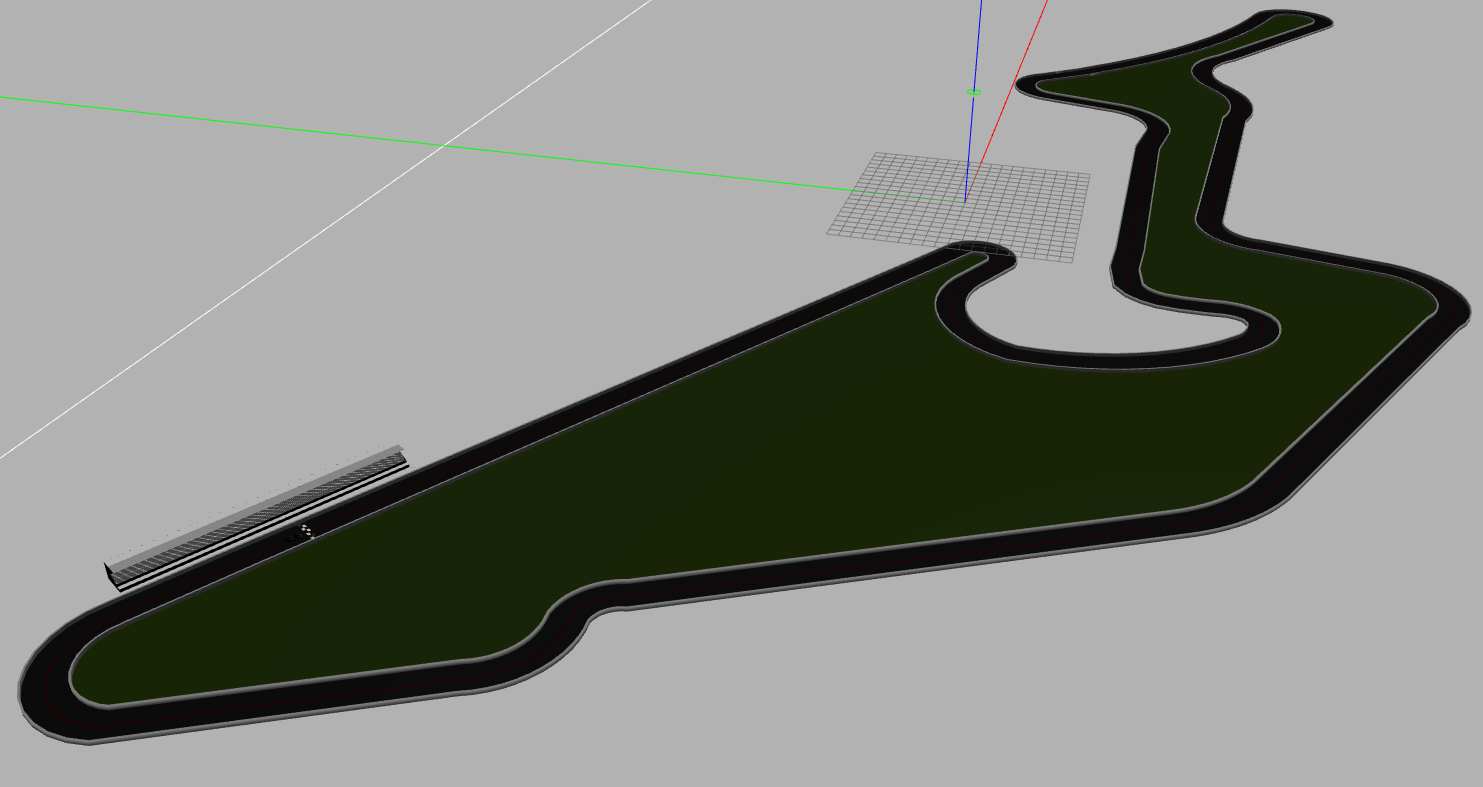
\includegraphics[width=0.95\textwidth, height=12cm]{figures/circuito.png}
		\caption{Modelo del circuito de Nürburging}
		\label{fig.circuito}
		\end{center}
\end{figure} 

\subsection{Ficheros de configuración} \label{sec.fichconf}
Para la incorporación del modelo del circuito y del robot, es necesario la creación de un modelo de configuración que importe en \textit{Gazebo} los elementos de los que consta el escenario y su localización. Este fichero tiene la extensión \textit{.world} y \textit{Gazebo} es capaz de leerlo y mostrar el escenario al iniciarse.
El código del fichero es el siguiente:

\lstset{language=XML, breaklines=true, basicstyle=\footnotesize}
\begin{lstlisting}[frame=single]
<?xml version="1.0"?>
<sdf version="1.4">
  <world name="default">
    <include>
      <uri>model://sun</uri>
    </include>
    <include>
      <uri>model://nurburgrinLine</uri>
      <pose>70 -47 0 0 0 0</pose>
    </include>
    <include>
      <uri>model://f1ROS</uri>
      <pose>0.05 -0.44 0 0 0 0.9</pose>
    </include>
  </world>
</sdf>
\end{lstlisting}

Además de este fichero de configuración, es necesario un fichero complementario que importe los \textit{plugins y drivers} de ROS-Kinetic. Este tipo de fichero tienen la extensión \textit{.launch}. En este fichero se pasan a \textit{Gazebo} argumentos como el nombre del fichero de configuración con el escenario, establecer el tiempo que se va a utilizar en el escenario, la posible implementación de un GUI y otras opciones de depuración.
El fichero es el siguiente:

\lstset{language=XML, breaklines=true, basicstyle=\footnotesize}
\begin{lstlisting}[frame=single]
<?xml version="1.0" encoding="UTF-8"?>
<launch>
  <!-- We resume the logic in empty_world.launch, changing only the name of the world to be launched -->
  <include file="$(find gazebo_ros)/launch/empty_world.launch">
    <arg name="world_name" value="nurburgrinLineROS.world"/> <!-- Note: the world_name is with respect to GAZEBO_RESOURCE_PATH environmental variable -->
    <arg name="paused" value="false"/>
    <arg name="use_sim_time" value="true"/>
    <arg name="gui" value="true"/>
    <arg name="headless" value="false"/>
    <arg name="debug" value="false"/>
    <arg name="verbose" default="false"/>
  </include>
</launch>
\end{lstlisting}

\section{Nodo Académico}
En esta sección se trata el desarrollo del nodo académico de la práctica (Figura 4.4). Este elemento ha sido desarrollado específicamente para la práctica ofreciendo al estudiante todas las herramientas necesarias para un desarrollo del algoritmo sencillo (Figura \ref{fig.na_ch}).

\begin{figure}[H]
  \begin{center}
    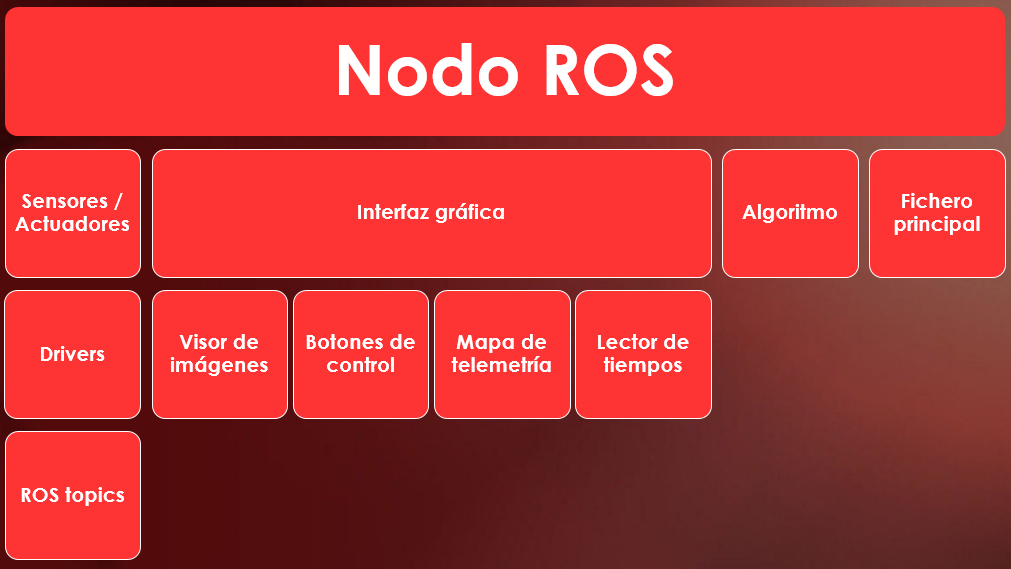
\includegraphics[width=0.5\textwidth, height=8cm]{figures/na_ch.png}
		\caption{Nodo Académico de Chrono}
		\label{fig.na_ch}
		\end{center}
\end{figure} 

\subsection{Arquitectura software}
Esta práctica tiene dos hilos de ejecución para aliviar la carga computacional de la práctica De esta manera se aumenta la velocidad  la que puede trabajar el simulador \textit{Gazebo}.

\begin{itemize}
	\item Hilo de sensores: este hilo se encarga de la actualización de los datos de los sensores del robot. Este hilo se comunica con \textit{Gazebo} para recoger datos de la odometría y la cámara y para publicar datos de control del motor para mover el robot.
	\item Hilo de la interfaz gráfica del usuario (GUI): este hilo se encarga del refresco del GUI de la práctica. En esta práctica tiene una carga computacional elevada dado se encarga de refrescar las imágenes obtenidas por la cámaras, el procesamiento visual sobre esa imagen que ha realizado el alumno, un mapa del circuito con la posición actualizada del robot y del robot fantasma a vencer, y una lectura controlada de tiempos para sincronizar ambos coches.
\end{itemize}

Gracias a esta interfaz gráfica el estudiante puede servirse de algunos elementos de depuración que veremos en profundidad en la sección 5.3.2 y 5.3.3. De esta manera el alumno solo tiene que centrarse en el desarrollo del algoritmo. El nodo académico dispone de una función reservada para que el alumno escriba su algoritmo en ella y pueda ver los resultados, todo ello viene indicado en fichero \textit{README.md} de la práctica.

\subsection{Interfaz de sensores y actuadores}
El nodo académico proporciona un API de sensores y actuadores al programador para facilitar la interconexión con los mismos. El API del robot es el siguiente:

\begin{itemize}
	\item \textit{self.pose3d.getPose3d()}: con esta función podemos obtener los datos de odometría y posición del robot.
	\item \textit{self.camera.getImage()}: con esta función se recogen las imágenes obtenidas por la cámara del robot.
	\item \textit{self.motors.senV() o self.motors.sendW()}: con esta función publicamos la velocidad y giro del robot.
\end{itemize}

\subsection{Interfaz gráfica}
La interfaz gráfica del usuario (GUI), se utiliza para representar información relacionada con los sensores del robot. Esta información es muy útil para la depuración del algoritmo del estudiante ya que permite la visualización de las publicaciones que realiza el algoritmo al robot.

Esta GUI (Figura \ref{fig.guich}) está formada por cuatro \textit{widgets}, uno para el visionado del robot, otro para su comportamiento, otro para su odometría y otro para la sincronización de la grabación de ROS con el nodo académico.

\begin{figure}[H]
  \begin{center}
    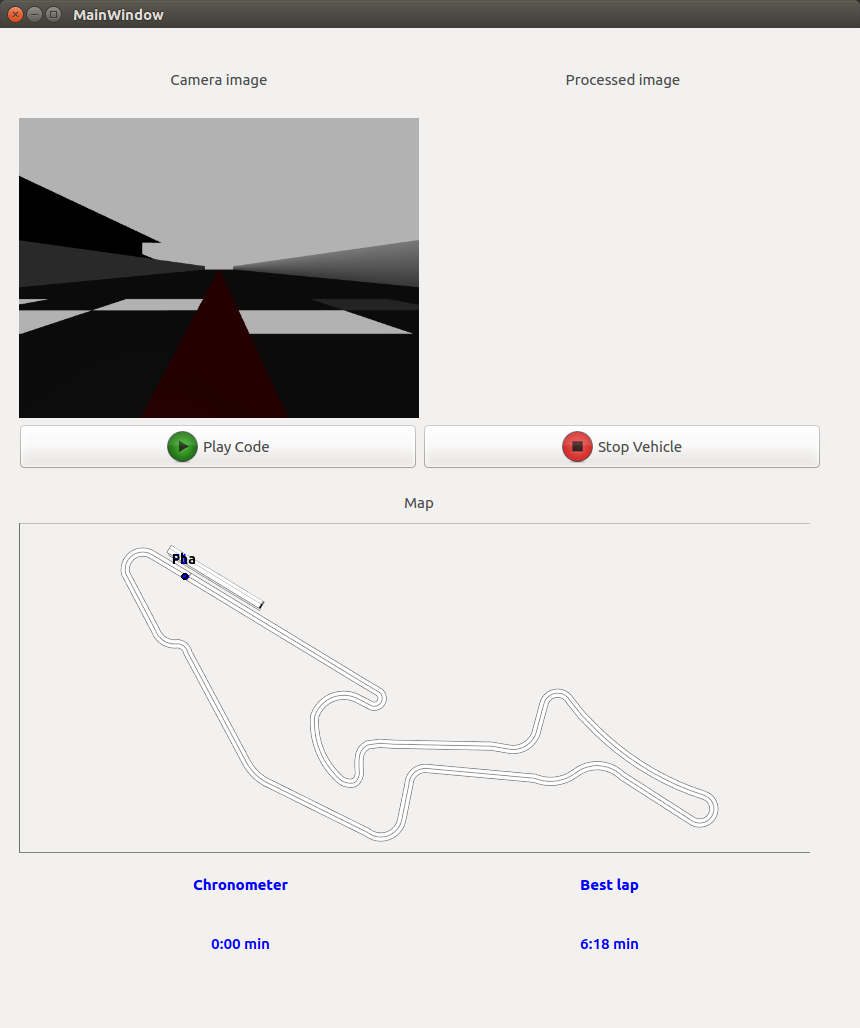
\includegraphics[width=7cm,height=10cm,\textwidth]{figures/GUI_Chrono.png}
		\caption{Interfaz Gráfica Chrono}
		\label{fig.guich}
		\end{center}
\end{figure}

El \textit{widget} superior recoge las imágenes captadas por la cámara del robot  y las muestra en una ventana del GUI. Al lado de las imágenes captadas por la cámara se muestra otra ventana con el filtrado que realice el alumno de esas imágenes. Esto es muy útil para el estudiante a la hora de enfrentarse al problema de visión que supone la primera parte de la solución de la práctica.

El tercer \textit{widget} está formado por un mapa del circuito, en este caso el circuito de Nürburgring, en el que se pueden visualizar las posiciones del robot y el robot fantasma con el récord del circuito.

El último \textit{widget} se llama \textit{ChronoWidget} y se trata de un algoritmo de de sincronización del tiempo de simulación de Gazebo con la reproducción a tiempo real de \textit{ROSbag}.

Además de estos \textit{widget}, en el GUI se incluyen distintos botones de control para hacer una pausa académica del algoritmo y para reiniciar la posición del teleoperador. El primer botón se llama \textit{pushButton} y consiste en un botón interactivo para iniciar el código programado por el alumno y para parar el código. El segundo botón se llama \textit{ResetButton} y se utiliza para reiniciar el teleoperador de la interfaz gráfica y hacer que el robot no se mueva.

La parte inferior del GUI tiene un lector de tiempos en el que se muestra el tiempo simulado de \textit{Gazebo} y, por lo tanto, el tiempo que está necesitando el robot para completar la vuelta. A su derecha se muestra el tiempo del récord del circuito para que el alumno tenga una idea de la optimización que necesita el código de control de movimiento del robot para que sea más eficiente.

\subsection{Visor de imágenes}
En este primer \textit{widget} se pueden visualizar las imágenes captadas por la cámara que incorpora el robot. Gracias a ella, el alumno puede tener una idea de la visión del robot y programar una solución de una manera más sencilla.

A la derecha de la ventana del visor de imágenes de la cámara, se ha incluido otra ventana de visualización. Esta ventana se encarga de mostrar el procesamiento de la imagen desarrollado por el alumno. Gracias a esta ventana, el alumno puede hacerse una idea del algoritmo de procesamiento de imagen que ha desarrollado.

\begin{figure}[H]
  \begin{center}
    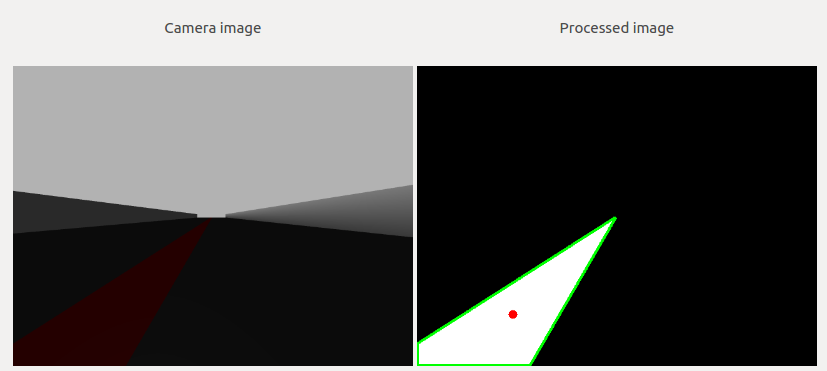
\includegraphics[width=0.98\textwidth]{figures/visor_imagen_chrono.png}
		\caption{Visor de imágenes de Chrono}
		\label{fig.vich}
		\end{center}
\end{figure}

\subsection{Botones de control}
Otra función incluida en el GUI son los botones de control. Existen dos botones de control ``Push Button''y ``Reset Button''.
Con el primer botón de control, se puede parar la ejecución de la práctica y volver a reanudarla. Con esto se permite un control en la depuración del código del alumno, ya que puede detener la ejecución en cualquier momento para visualizar los datos que seestáan recogiendo.

El segundo botón es complementario al primero, pues su funcionalidad es la de reiniciar las publicaciones de datos que se envian a los motores del robot. Es decir, con este botón se puede parar el robot y después con el botón ``Push Button'' se puede parar la ejecución.

\begin{figure}[H]
	\begin{center}
	    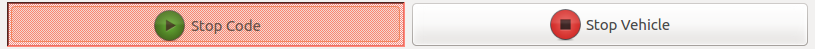
\includegraphics[width=0.98\textwidth]{figures/boton_pausa_chrono.png}
		\caption{Ilustración del botón de pausa académica}
		\label{fig.bpch}
	\end{center}
\end{figure}
\begin{figure}[H]
	\begin{center}
        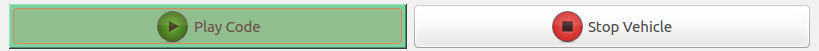
\includegraphics[width=0.98\textwidth]{figures/boton_start_chrono.png}
		\captionof{figure}{Ilustración del botón de comienzo académico}
		\label{fig.bsch}
	\end{center}
\end{figure}


\subsection{Mapa de odometría}
Ya se ha descrito la funcionalidad del mapa en la sección anterior, en esta sección nos vamos a centrar en el algoritmo que dota de esta funcionalidad al mapa.

El nodo académico, concretamente el hilo de ejecución encargado del interfaz gráfico (GUI), se encarga de cargar la imagen del mapa en el GUI. Una vez hecho esto, recoge los datos de odometría del sensor \textit{Pose3D} y dibuja su posición en el mapa. Adicionalmente, recoge los datos de odometría del fichero de grabación de ROS para extraer la posición del coche fantasma y dibujarla en el mapa también.

\begin{figure}[H]
  \begin{center}
    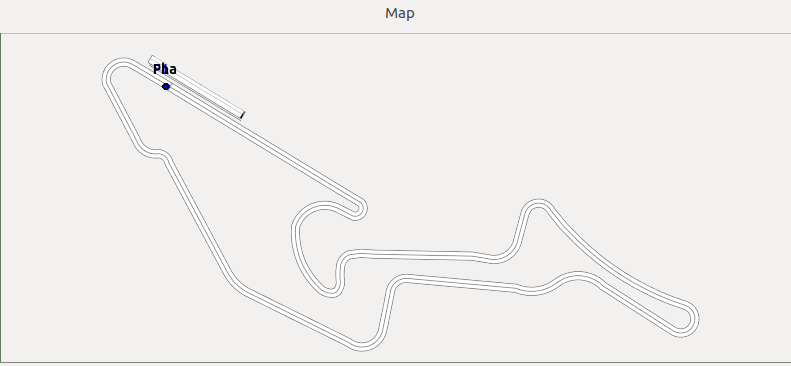
\includegraphics[width=0.98\textwidth]{figures/mapa_chrono.png}
		\caption{Mapa del GUI}
		\label{fig.mapach}
		\end{center}
\end{figure}

Esta ejecución es bastante pesada dado que requiere de una actualización constante para reflejar una posición lo más exacta posible, tanto del coche fantasma como del robot. Es por ello que se utiliza el hilo de ejecución proporcionado por el GUI. Esto alivia a la ejecución principal de una gran carga computacional.

\subsection{Lector de tiempos}
Este ha sido el principal reto de esta práctica por su complejidad a la hora de recoger los datos, tanto de \textit{Gazebo}, como de \textit{ROSbag} y sincronizarlos.

El problema que se planteaba en la sincronización de tiempos era el hecho de que los tiempos de \textit{Gazebo} se sincronizan mediante el tiempo de simulación del propio simulador pero los tiempos grabados de \textit{Gazebo} mediante ROSbag, se reproduce mediante el tiempo real. Esto supone una desincronización muy grande ya que, en el tiempo de simulación es, aproximadamente, un 0,15 veces el tiempo real. Adicionalmente existe el problema de que el tiempo de simulación depende de la potencia de cómputo de cada ordenador, por lo que la reproducción no se puede realizar a  un ritmo constante porque sería un hándicap muy grande para los ordenadores potentes que se verían afectados a reproducir de una manera muy lenta.

En este aspecto, debían abordarse los dos problemas propuestos de manera simultánea. Por un lado sincronizar el tiempo de reproducción con el tiempo de simulación, y por otro llevar un ritmo del tiempo de simulación adaptado para la carga de cómputo que pueda soportar cada ordenador. Adicionalmente se encontró un problema adicional con la reproducción de la grabación de ROSbag por el cual, las etiquetas de tiempo de las que consta, no se inicializan desde el comienzo sino que se graban con el tiempo simulado actual. Es por esto que la reproducción comienza con una etiqueta temporal distinta de cero.

Para solucionar sendos problemas ha sido necesaria la definición de diversas medidas de tiempos:

\begin{itemize}
	\item \textit{Tiempo de grabación}: este tiempo representa el ritmo al que se reproduce la grabación de ROSbag.
	\item \textit{Tiempo simulado}: este tiempo representa el tiempo al que se refresca el simulador \textit{Gazebo}.
	\item \textit{Tiempo de reproducción}: este tiempo se basa en el tiempo de simulación pero restándole el offset del comienzo de la práctica. Por ello empieza cuando el estudiante ejecuta la práctica en lugar de cuando se inicia el simulador.
\end{itemize}

El algoritmo de simulación comienza recogiendo el instante de tiempo en el que el alumno ejecuta su código mediante el comando:

\lstset{language=Python, breaklines=true, basicstyle=\footnotesize}
\begin{lstlisting}[frame=single]
initime = rospy.Time.from_sec(rospy.get_time()).to_sec()
\end{lstlisting}

Una vez obtenido el tiempo inicial, es necesario recoger el instante de tiempo en el que estamos refrescando la sincronización:

\lstset{language=Python, breaklines=true, basicstyle=\footnotesize}
\begin{lstlisting}[frame=single]
sim_time = rospy.Time.from_sec(rospy.get_time()).to_sec()
\end{lstlisting}

Además de estos dos tiempos, es necesario conocer el tiempo de la primera etiqueta de la grabación de ROSbag para comenzar a leer las etiquetas desde ese offset:
\lstset{language=Python, breaklines=true, basicstyle=\footnotesize}
\begin{lstlisting}[frame=single]
rep_start = str(bag).split('start:       ')[1].split(' ')[4].split()[0][1:-1]
\end{lstlisting}
Con el tiempo de simulación actual, el tiempo inicial y el tiempo de inicio de la reproducción, podemos obtener el tiempo con el que vamos a comparar las etiquetas temporales de la grabación para saber si tenemos que leer la etiqueta temporal y actualizar la posición del coche fantasma en el mapa del GUI o seguir devolviendo la misma posición porque es pronto.

\lstset{language=Python, breaklines=true, basicstyle=\footnotesize}
\begin{lstlisting}[frame=single]
t_sim_unif = sim_time - initime + float(rep_start)
\end{lstlisting}

Gracias a esta sincronización se pueden devolver los valores de odometría grabados para la solución con el récord de la vuelta para el coche fantasma y actualizar su posición en el mapa. A continuación se describe el código utilizado para la sincronización:

\lstset{language=Python, breaklines=true, basicstyle=\footnotesize}
\begin{lstlisting}[frame=single]
def synchronize(self):
        global posx, posy, cursor

        t_sim_unif = sim_time - initime + float(rep_start)
        if initime != 0.0 and t_sim_unif != 0.0:
            for (topic,msg,t) in bag.read_messages(start_time=rospy.Time(t_sim_unif-0.05)):
                t = t.to_sec()
                if t_sim_unif > t:
                    try:
                        posx = str(msg).split('x: ')[1].split()[0]
                        posy = str(msg).split('y: ')[1].split()[0]
                        return float(posx), float(posy)
                    except IndexError:
                        pass
                else:
                    return float(posx), float(posy)

        else:
            return float(posx), float(posy)
\end{lstlisting}

A continuación se muestra una imagen (Figura \ref{fig.ltch}) del \textit{widget} en el GUI con la práctica iniciada. A la izquierda se puede visualizar el chronómetro con la duración de la ejecución y a su derecha se encuentra el registra con el la duración de la vuelta para la grabación que se esté reproduciendo.

\begin{figure}[H]
  \begin{center}
    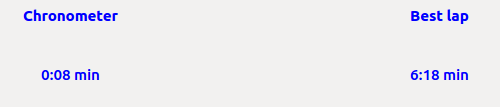
\includegraphics[width=0.98\textwidth]{figures/lector_tiempos_chrono.png}
		\caption{Lector de tiempos de Chrono}
		\label{fig.ltch}
		\end{center}
\end{figure}

\section{Soluciones de referencia}
Para la práctica, ha sido necesario el desarrollo de dos soluciones de referencia distintas. Una de ellas ha sido adaptada de una solución previamente hecha y la otra solución ha sido programada por completo.

La primera solución ha sido adaptada de otra práctica de \textit{JdeRobot Academy} llamada \textit{Follow Line}. Aunque esta práctica es similar, la solución estaba desactualizada por lo que ha sido necesaria una actualización del código, en específico de la parte de comparación de píxeles en la imagen filtrada y de la parte de control de movimiento. La actualización de la parte del control de movimiento ha sido más completa debido a que la velocidad del coche en las curvas era demasiado elevada y no estaba sincronizada con el refresco y filtrado de imagen que realiza la cámara insertada en el coche de 20 imágenes por segundo.

La segunda solución desarrollada, ha sido creada por completo utilizando la librería \textit{OpenCV}, con funciones \textit{Built-in} proporcionadas por la misma que facilitan la comprensión del código programado. Para ello ha sido necesario un estudio más profundo de esta librería que ha dotado de la inteligencia necesaria para reescribir el filtrado de imagen en un algoritmo mucho más eficiente y que permite un procesamiento de las imágenes más elevado. Gracias a esto, la velocidad del robot es mayor y por consiguiente, completa la vuelta al circuito sin colisiones y en un tiempo menor.

\subsection{Procesamiento de imagen} \label{sec.pdi}
El procesamiento de la imagen captada por la cámara, comienza con la recogida de la imagen guardada en el búffer de la misma con la instrucción:

\lstset{language=Python, breaklines=true, basicstyle=\footnotesize}
\begin{lstlisting}[frame=single]
input_image = self.camera.getImage().data
\end{lstlisting}

Gracias a esta instrucción es posible ver la imagen captada en la interfaz gráfica del usuario.

Una vez obtenida la imagen, hay que transformarla a una imagen HSV\footnote{\url{https://es.wikipedia.org/wiki/Modelo_de_color_HSV}} para poder seleccionar el color rojo de la línea central del circuito:

\lstset{language=Python, breaklines=true, basicstyle=\footnotesize}
\begin{lstlisting}[frame=single]
image_HSV = cv2.cvtColor(input_image, cv2.COLOR_RGB2HSV)
\end{lstlisting}

Tras obtener la imagen HSV, podemos seleccionar el rango de valores que componen el rojo de la línea como un array con la intensidad mínima y máxima del color.

\lstset{language=Python, breaklines=true, basicstyle=\footnotesize}
\begin{lstlisting}[frame=single]
value_min_HSV = np.array([0, 150, 0])
value_max_HSV = np.array([180, 255, 255])
\end{lstlisting}

Con esos valores realizamos un filtrado de la imagen para obtener la línea roja exclusivamente:

\lstset{language=Python, breaklines=true, basicstyle=\footnotesize}
\begin{lstlisting}[frame=single]
image_HSV_filtered = cv2.inRange(image_HSV, value_min_HSV, value_max_HSV)
\end{lstlisting}

Usamos el filtro obtenido como una máscara para filtrar la imagen y obtener de esta forma la imagen filtrada en blanc y negro. De esta manera el blanco serán los colores que pasen el filtro y en negro obtendremos el resto de colores. En este caso, obtendremos la líneaa roja del circuito en color blanco y el resto de la imagen en negro:

\lstset{language=Python, breaklines=true, basicstyle=\footnotesize}
\begin{lstlisting}[frame=single]
image_HSV_filtered_Mask = np.dstack((image_HSV_filtered, image_HSV_filtered, image_HSV_filtered))
\end{lstlisting}

Una vez filtrada la imagen, se procede a obtener los contornos de la zona filtrada. Para ello, es necesario convertir la imagen a escala de grises:

\lstset{language=Python, breaklines=true, basicstyle=\footnotesize}
\begin{lstlisting}[frame=single]
imgray = cv2.cvtColor(image_HSV_filtered_Mask, cv2.COLOR_BGR2GRAY)
\end{lstlisting}

De esta manera, se pueden conseguir los píxeles que tiene un contraste mayor con sus vecinos, obteniendo el contorno:

\lstset{language=Python, breaklines=true, basicstyle=\footnotesize}
\begin{lstlisting}[frame=single]
ret, thresh = cv2.threshold(imgray, 127, 255, 0)
_, contours, hierarchy = cv2.findContours(thresh, cv2.RETR_TREE, cv2.CHAIN_APPROX_SIMPLE)
\end{lstlisting}

Una vez conseguido el contorno, se dibuja en la imagen filtrada:

\lstset{language=Python, breaklines=true, basicstyle=\footnotesize}
\begin{lstlisting}[frame=single]
cv2.drawContours(image_HSV_filtered_Mask, contours, -1, (0,255,0), 3)
\end{lstlisting}

El siguiente algoritmo, una vez realizado el filtro, es para robustecer el código en el caso de que, en el filtrado de la imagen, se detecten dos zonas con filtro. Esto se puede producir cuando hay una curva y, debido a la resolución de la cámara, recoge la línea roja pero incompleta. Esto produce lagunas de filtro en las que no se visualiza la línea por completo, sino cortada. Para evitar un fallo en el algoritmo, ha sido necesaria la inclusión del siguiente código que recoge todas las zonas filtradas y selecciona la de mayor área:

\lstset{language=Python, breaklines=true, basicstyle=\footnotesize}
\begin{lstlisting}[frame=single]
area = []
for pic, contour in enumerate(contours):
    area.append(cv2.contourArea(contour))
if len(area) > 1:
    if area[0] < area[1]:
        M = cv2.moments(contours[1])
    else:
        M = cv2.moments(contours[0])
else:
    M = cv2.moments(contours[0])
\end{lstlisting}

Tras esta comprobación, se obtienen los valores de los ejxes x e y de la zona filtrada. Estos valores forman el centro del área que ha sido filtrada:

\lstset{language=Python, breaklines=true, basicstyle=\footnotesize}
\begin{lstlisting}[frame=single]
if int(M['m00']) != 0:
    self.cx = int(M['m10']/M['m00'])
    self.cy = int(M['m01']/M['m00'])
\end{lstlisting}

Gracias a estos valores, en concreto al valor del eje x, podemos saber la diferencia de posición que tiene el robot con el centro de la línea roja, es decir, la diferencia de posición del robot con el centro del circuito. Para facilitar este cálculo, se ha dibujado un punto en la imagen filtrada con los valores del eje y el eje y para que sea visualizado:

\lstset{language=Python, breaklines=true, basicstyle=\footnotesize}
\begin{lstlisting}[frame=single]
cv2.circle(image_HSV_filtered_Mask, (self.cx, self.cy), 7, np.array([255, 0, 0]), -1)
\end{lstlisting}

Para la visualización de la imagen procesada, basta con utilizar la instrucción proporcionada por la interfaz gráfica del usuario:

\lstset{language=Python, breaklines=true, basicstyle=\footnotesize}
\begin{lstlisting}[frame=single]
self.setImageFiltered(image_HSV_filtered_Mask)
\end{lstlisting}

\subsection{Control de movimiento}
En esta sección vamos a tratar el control del movimiento del robot. Es una parte compleja ya que supone un filtrado correcto. En caso contrario, el comportamiento del movimiento del robot será incorrecto. Esto es debido a que el movimiento del robot se realiza en consecuencia al procesamiento de la imagen.

\subsubsection{Filtrado de imagen y control de movimiento basado en píxeles} \label{subsec.ficmbp}
Este tipo de control de movimiento se basa en la primera solución de la práctica y supone una transformación de la imagen a blanco y negro, para después comprobar los píxeles que cambian de tono para saber hacia qué lado hay que orientar al coche.
Se trata de una solución eficaz aunque poco eficiente. Esto es debido a que es necesario comprobar los píxeles uno a uno para averiguar qué píxeles son los que han sufrido esta transformación de tono:

\lstset{language=Python, breaklines=true, basicstyle=\footnotesize}
\begin{lstlisting}[frame=single]
# Shape gives us the number of rows and columns of an image
size = image.shape
rows = size[0]
columns = size[1]

#  Looking for pixels that change of tone
position_pixel_left = []
position_pixel_right  = []

for i in range(0, columns-1):
    value = image_HSV_filtered[365, i] - image_HSV_filtered[365, i-1]
    if(value != 0):
        if (value == 255):
            position_pixel_left.append(i)
        else:
            position_pixel_right.append(i-1)


# Calculating the intermediate position of the road
if ((len(position_pixel_left) != 0) and (len(position_pixel_right) != 0)):
    position_middle = (position_pixel_left[0] + position_pixel_right[0]) / 2
elif ((len(position_pixel_left) != 0) and (len(position_pixel_right) == 0)):
    position_middle = (position_pixel_left[0] + columns) / 2
elif ((len(position_pixel_left) == 0) and (len(position_pixel_right) != 0)):
    position_middle = (0 + position_pixel_right[0]) / 2
else:
    position_pixel_right.append(1000)
    position_pixel_left.append(1000)
    position_middle = (position_pixel_left[0] + position_pixel_right[0])/ 2

# Calculating the desviation
desviation = position_middle - (columns/2)
\end{lstlisting}

Una vez obtenidos estos píxeles, el control de movimiento se ejecuta según el siguiente algoritmo, que comprueba estos píxeles y se mueve en consecuencia:

\lstset{language=Python, breaklines=true, basicstyle=\footnotesize}
\begin{lstlisting}[frame=single]
if (desviation == 0):
     self.motors.sendV(3)
elif (position_pixel_right[0] == 1000):
     self.motors.sendW(-0.0000035)
elif ((abs(desviation)) < 85):
     if ((abs(desviation)) < 31):
         self.motors.sendV(3)
     else:
         self.motors.sendV(1)
     self.motors.sendW(-0.000045 * desviation)
elif ((abs(desviation)) < 150):
     if ((abs(desviation)) < 120):
         self.motors.sendV(1)
     else:
         self.motors.sendV(1)
     self.motors.sendW(-0.00045 * desviation)
else:
     self.motors.sendV(1)
     self.motors.sendW(-0.0055 * desviation)
\end{lstlisting}

\subsubsection{Filtrado de imagen y control de movimiento basado en el centro del contorno}
Este tipo de filtrado de imagen es el descrito en la sección \ref{sec.pdi} y es mucho más eficiente y con una eficacia mayor que el descrito en el apartado anterior\ref{subsec.ficmbp}. Esto es debido a que no necesita comprobar la imagen completa píxel a píxel, sino que filtra el área de la línea y procesa su centro.

Una vez hecho este filtro, la control de movimiento es sencillo, pues basta con obtener el valor del eje x cuando el coche está alineado con la línea recta y tomarlo como el movimiento nulo. Tras esto, se puede definir el giro del robot en consonancia con este valor de movimiento nulo.
Gracias a ello, el robot girará más o menos cuanto mayor sea la diferencia entre el valor de movimiento nulo (153 aproximadamente) y el valor actual del eje x:

\lstset{language=Python, breaklines=true, basicstyle=\footnotesize}
\begin{lstlisting}[frame=single]
if self.cx < 50:
    self.motors.sendV(1.5)
else:
    self.motors.sendV(3.5)

self.motors.sendW((153-int(self.cx))*0.01)
\end{lstlisting}

\section{Experimentación}
La optimización de los algoritmos anteriores ha sido posible gracias a la realización de diversos experimentos. Estos experimentos han hecho salir a la luz errores en el algoritmo desarrollado que han sido subsanados.

Además se han realizado experimentos globales donde se ha testeado la práctica en su totalidad, nodo académico, infraestructura de la práctica y solución desarrollada.

\subsection{Ejecución típica}
Se ha preparado un documento \textit{README.md}, incluido en la infraestructura de la práctica, que sirve de guía al alumno a la hora de ejecutar la práctica. En él se incluye información acerca de su ejecución, la API de los sensores y actuadores de ROS e, incluso, un vídeo demostrativo con una ejecución.

Para ejecutar al práctica, es necesario lanzar en una terminal el fichero de configuración de ROS, llamado \textit{f1-chrono.launch}, descrito en la sección \ref{sec.fichconf}. Para lanzar el fichero hay que ejecutar el siguiente comando:

\lstset{language=bash, breaklines=true, basicstyle=\footnotesize}
\begin{lstlisting}[frame=single]
roslaunch f1-chrono.launch
\end{lstlisting}

Una vez lanzado el comando en la terminal, se abrirá el simulador \textit{Gazebo} con el escenario del circuito (Figura \ref{fig.circuito}).

\begin{figure}[H]
  \begin{center}
    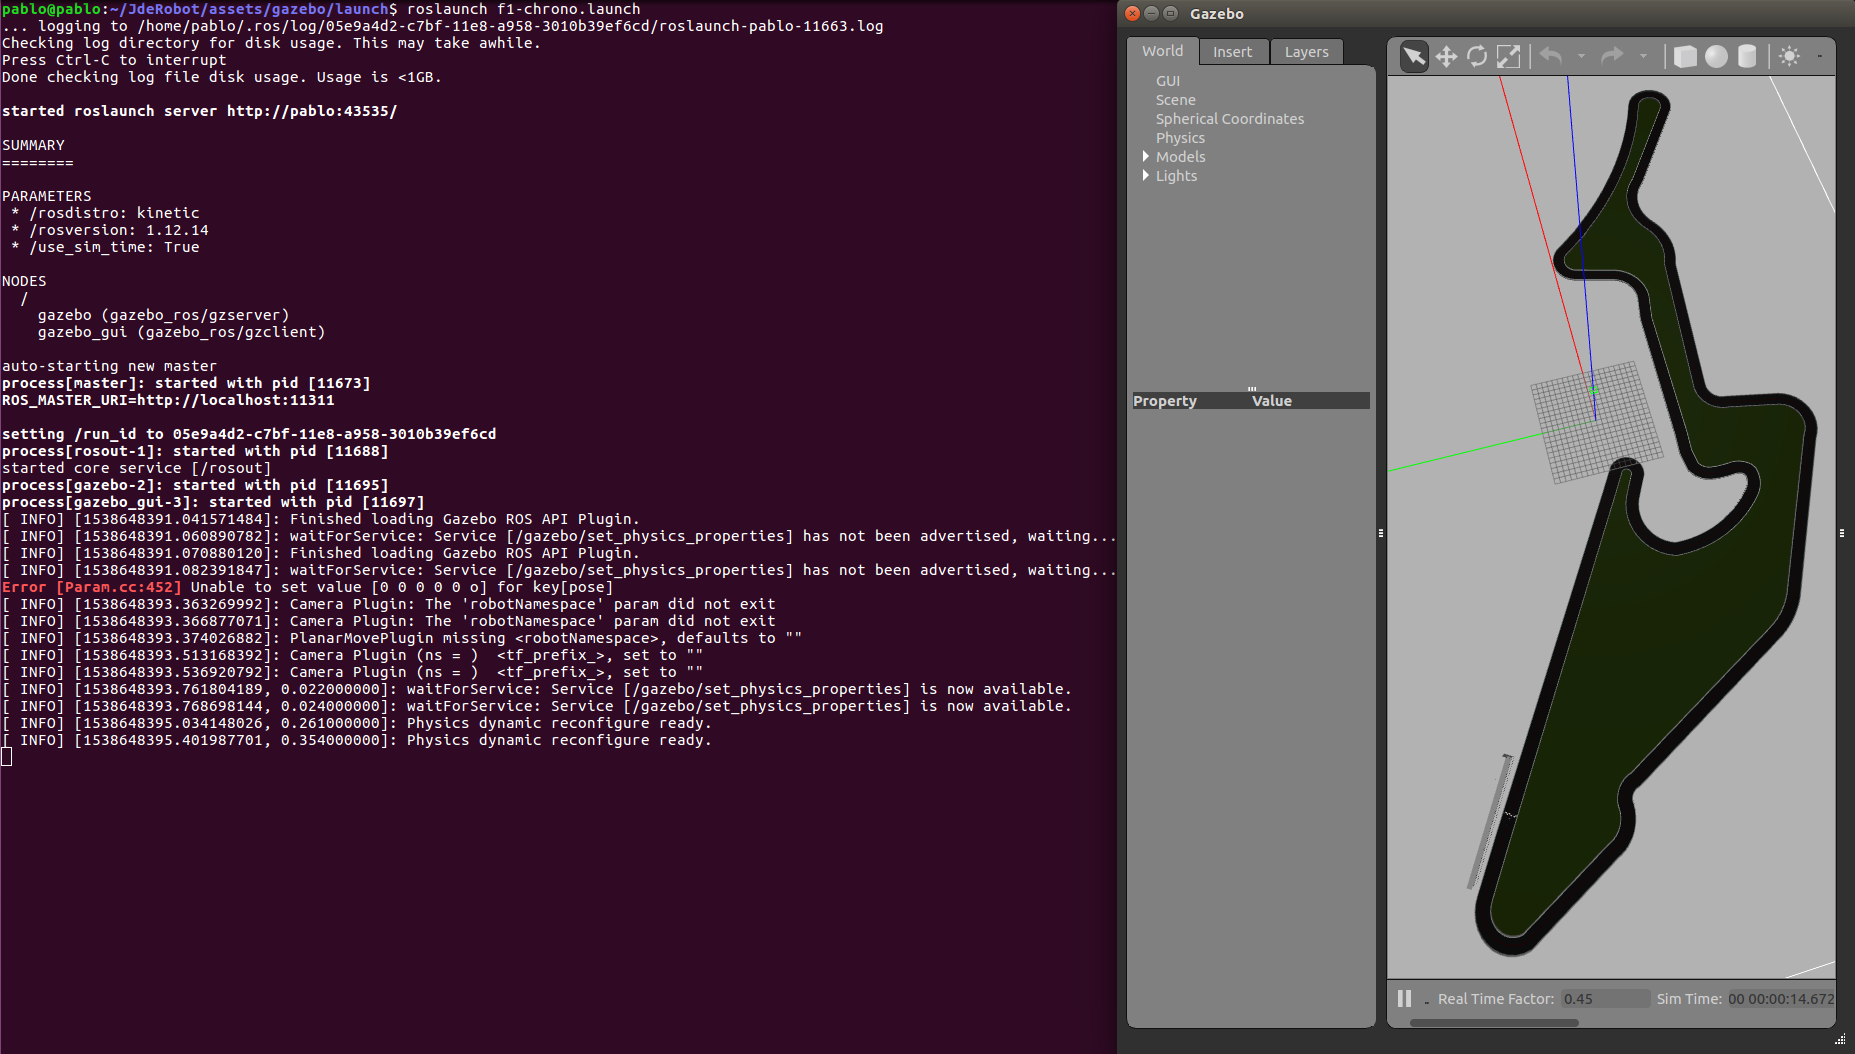
\includegraphics[width=0.98\textwidth]{figures/roslaunch_chrono.png}
		\caption{Inicialización ROS y Gazebo}
		\label{fig.roslaunchch}
		\end{center}
\end{figure}

Para iniciar el componente académico, será necesario ejecutar otro comando en una terminal distinta:

\lstset{language=bash, breaklines=true, basicstyle=\footnotesize}
\begin{lstlisting}[frame=single]
cd ~/Academy/exercises/chrono
python2 chrono.py
\end{lstlisting}

Una vez ejecutado el comando, el componente académico enlazará los sensores y actuadores proporcionados por \textit{ROS-Kinetic} mediante el fichero de configuración lanzado previamente a las variables:

\begin{itemize}
    \item self.camera
    \item self.pose3d
    \item self.motors
\end{itemize}

Con estas variables, el nodo académico se comunica con los \textit{drivers} de \textit{ROS-Kinetic}.
Además de realizar la conexión con los sensores y actuadores, al ejecutar la instrucción, nos aparecerá la interfaz gráfica de usuario (GUI) en la que se podrá visualizar las imágenes recogidas por la cámara, los botones de control, el mapa del circuito y el lector de tiempos (Figura \ref{fig.inaGch}).

\begin{figure}[H]
  \begin{center}
    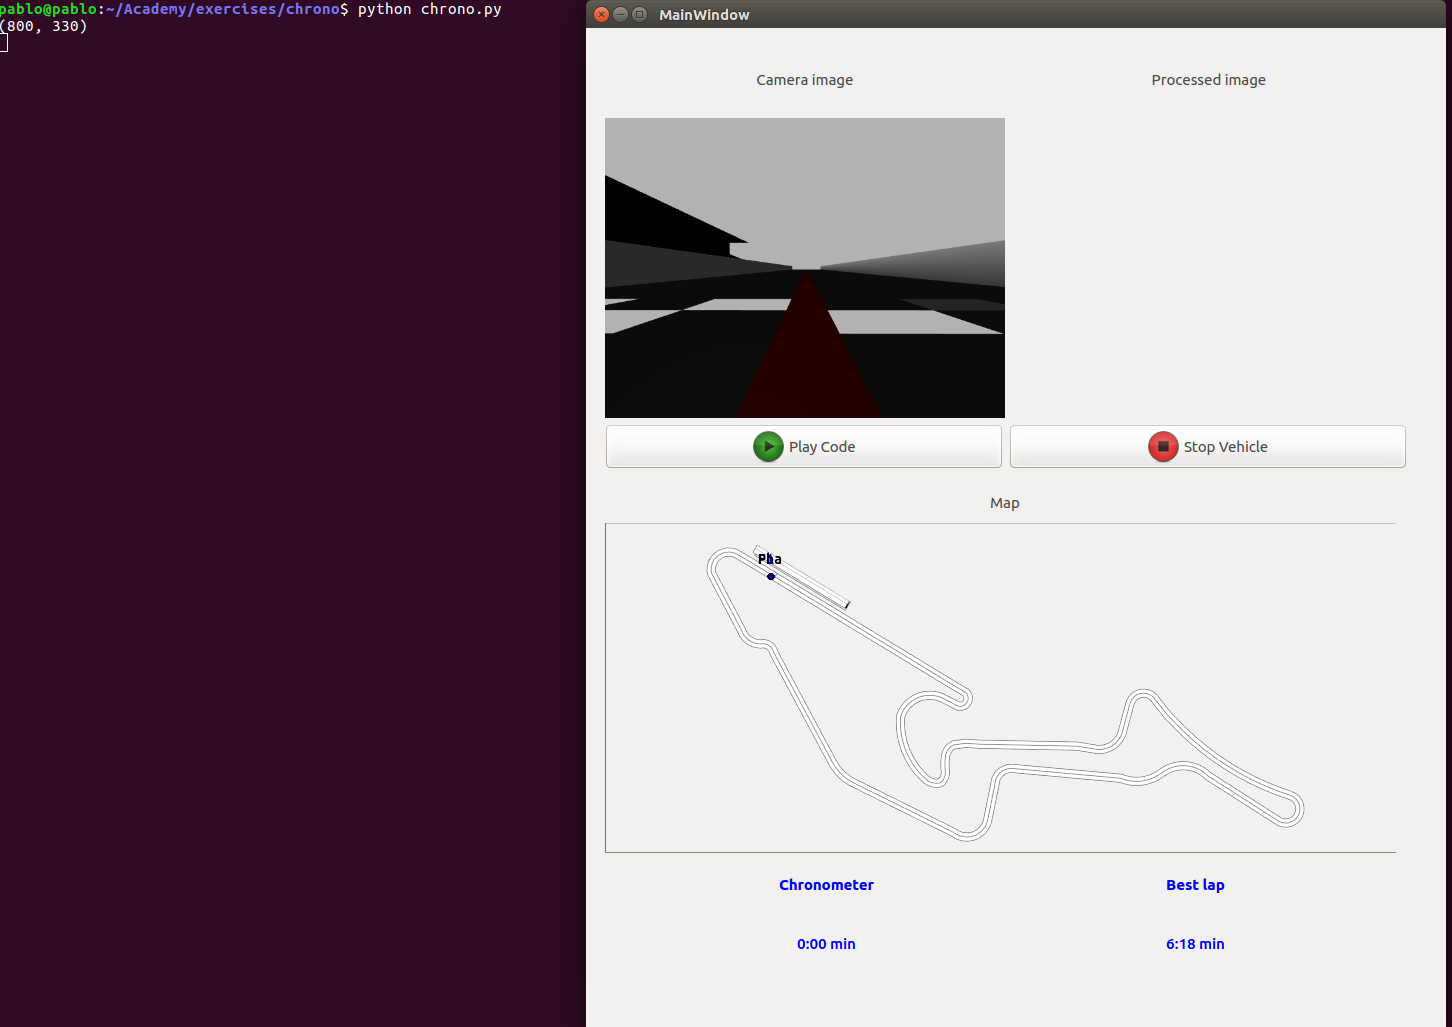
\includegraphics[width=0.98\textwidth]{figures/init_na_chrono.png}
		\caption{Inicialización del nodo académico y el GUI}
		\label{fig.inaGch}
		\end{center}
\end{figure}

Una vez inicializados los \textit{drivers de ROS-Kinetic}, el escenario en el simulador y el nodo académico, con su GUI, se puede iniciar el algoritmo desarrollado por el alumno pulsando sobre el botón ``Play Code''. De esta manera, la lógica programada podrá ser visualizada tanto en el GUI, como en el simulador.
 
\subsection{Ejecución estática}
En el caso en el que el alumno no programe el control de movimiento en su algoritmo, es posible ejecutar el código de igual manera. Esto es útil para depurar el algoritmo de procesamiento de imagen. 

El alumno tiene dos opciones en este aspecto. La primera consiste en dejar el robot inmóvil y ver el procesamiento realizado en la ventana para la imagen procesada del GUI. 

\begin{figure}[H]
  \begin{center}
    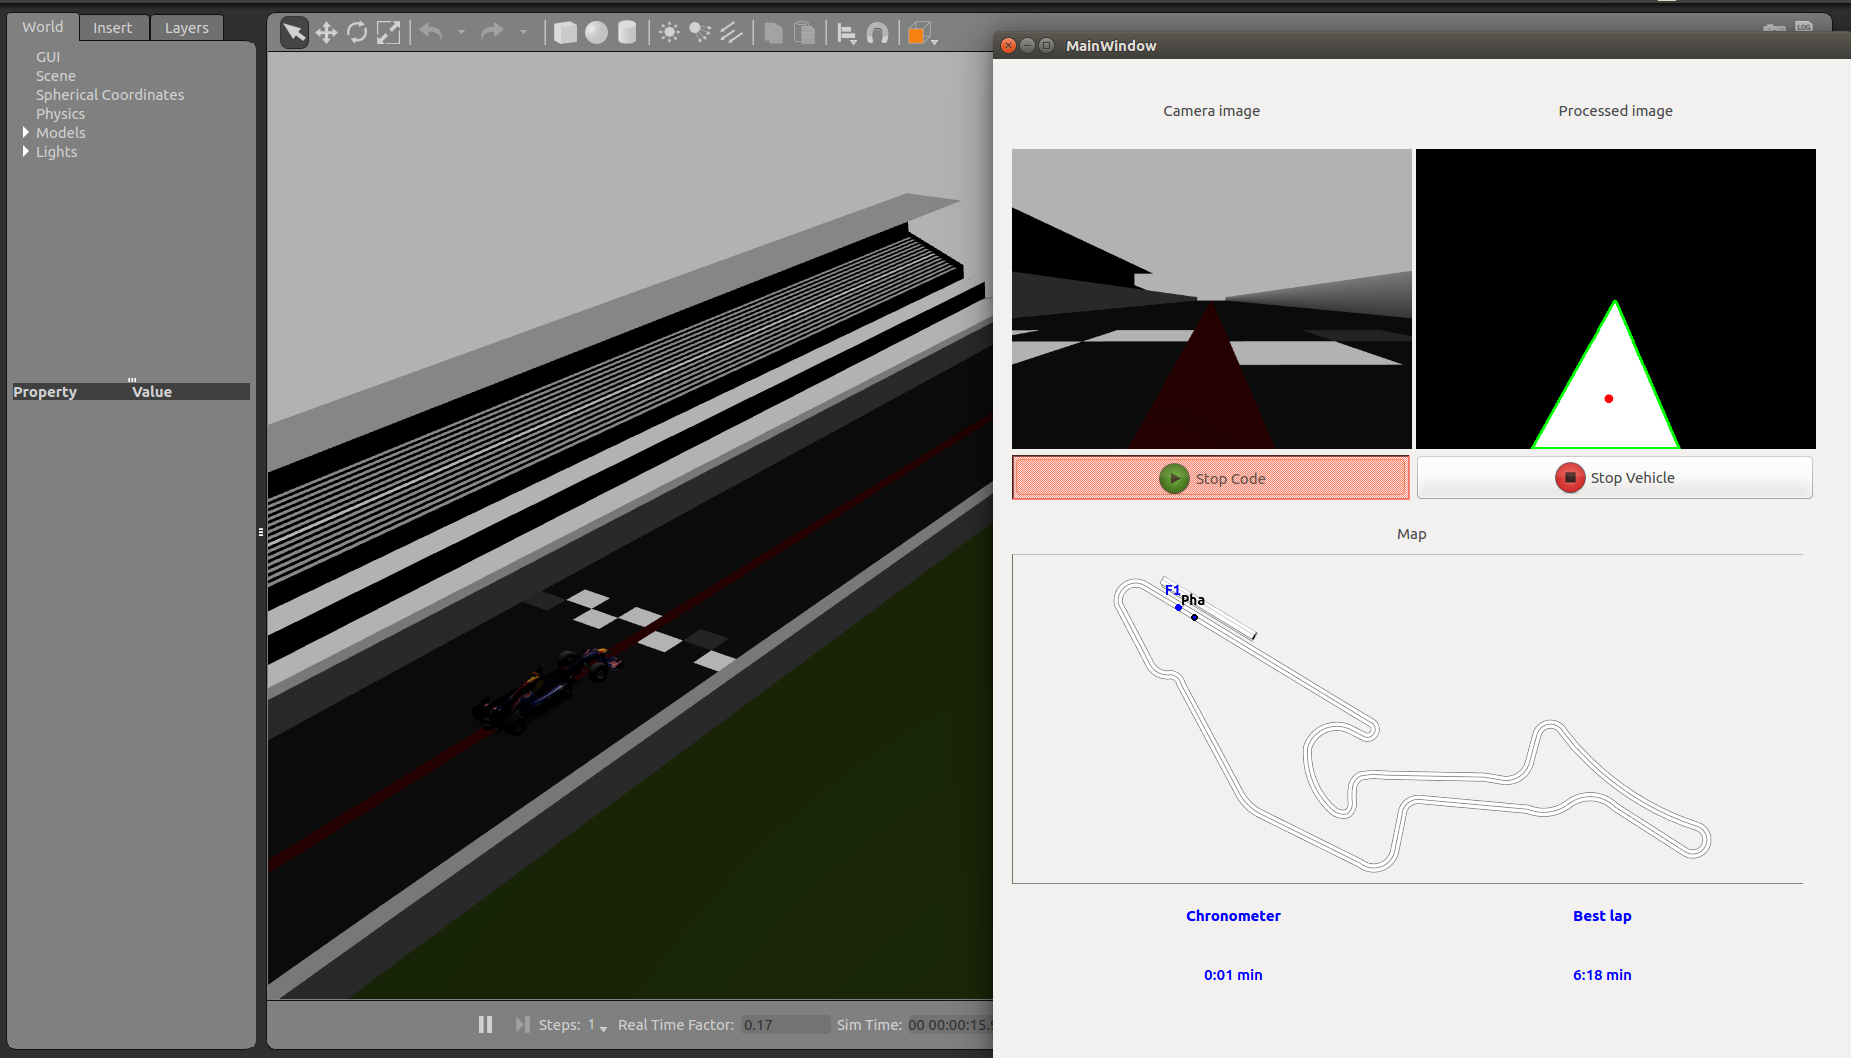
\includegraphics[width=0.98\textwidth]{figures/ejec_estat_chrono.png}
		\caption{Ejecución estática de la práctica}
		\label{fig.eech}
		\end{center}
\end{figure}

Otra opción, una vez haya superado esa primera prueba, es seleccionar una velocidad fija para mover el robot y visualizar el filtrado en movimiento.

\lstset{language=Python, breaklines=true, basicstyle=\footnotesize}
\begin{lstlisting}[frame=single]
self.motors.sendV(1)
\end{lstlisting}

\begin{figure}[H]
  \begin{center}
    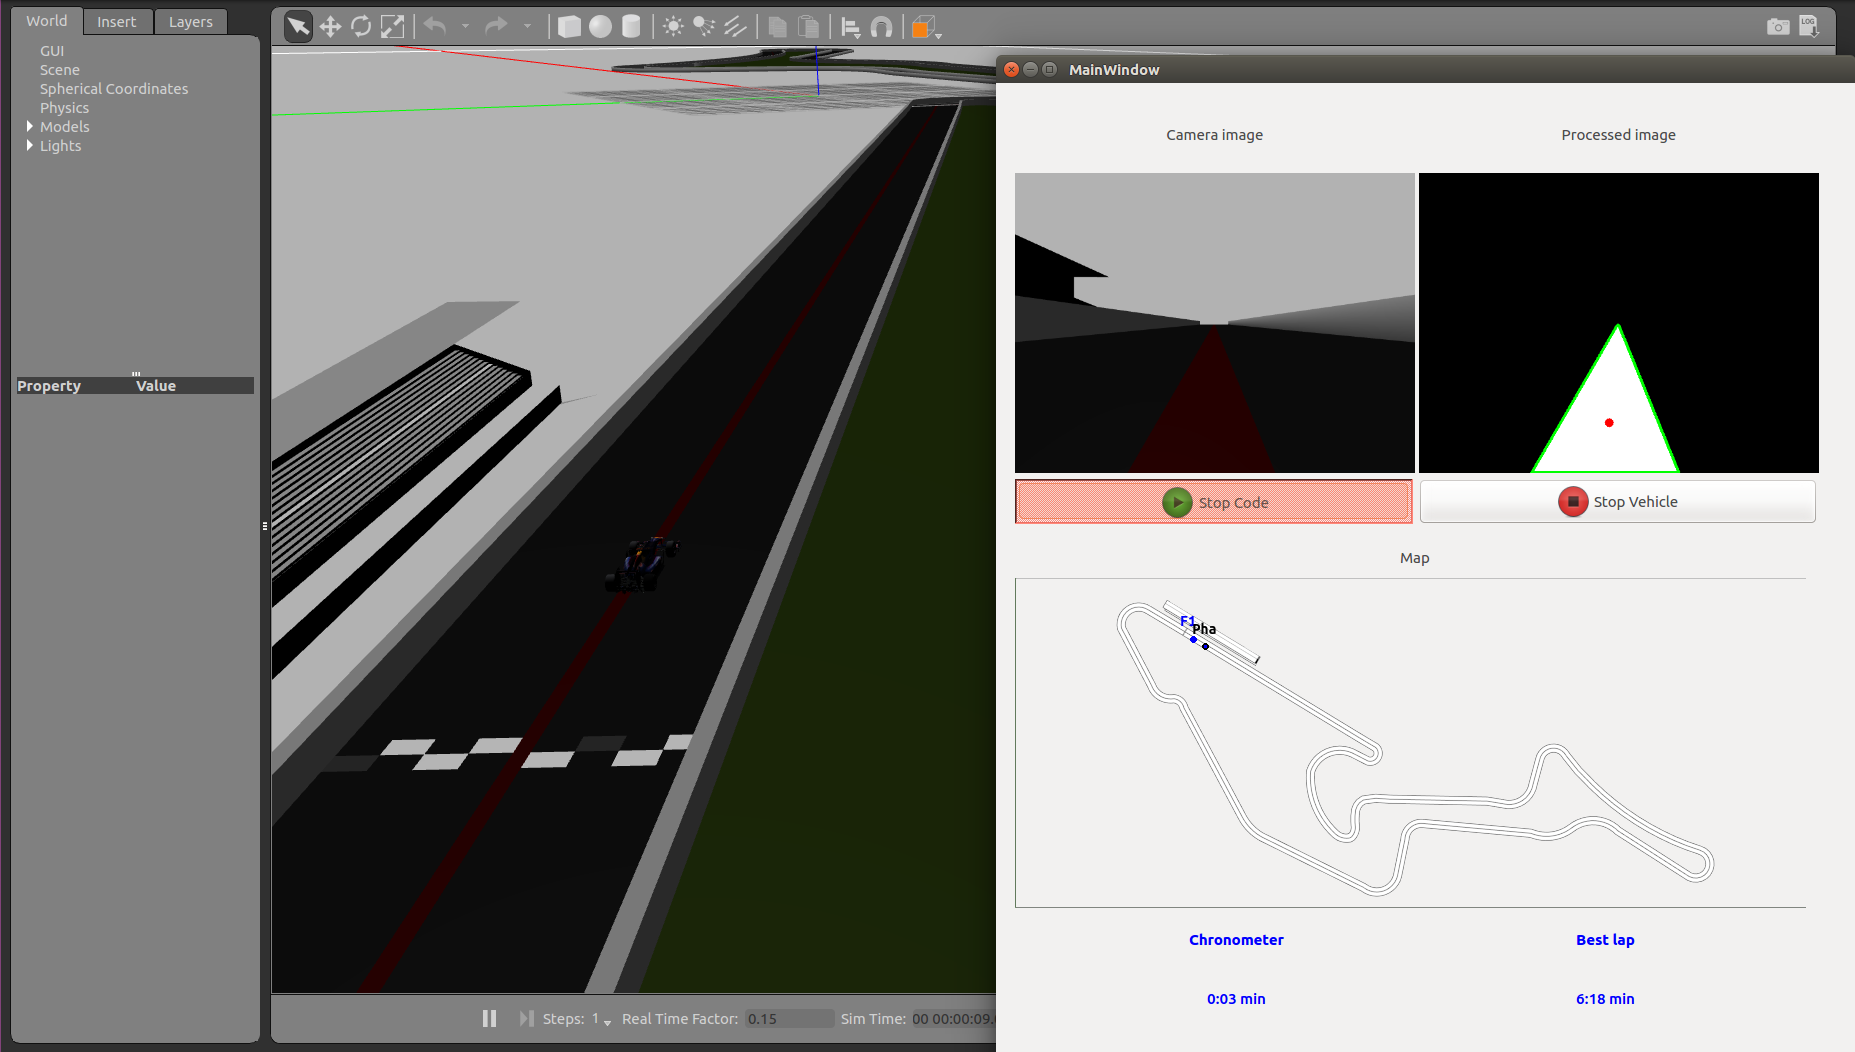
\includegraphics[width=0.98\textwidth]{figures/ejec_semiestat_chrono.png}
		\caption{Ejecución con velocidad fija}
		\label{fig.esech}
		\end{center}
\end{figure}

Con esta ejecución semi-móvil de la práctica, el alumno también puede visualizar, no solo la odometría del fantasma, que se visualizará cada vez que se ejecute el algoritmo, sino la odometría del robot a programar. Con esto, el alumno se puede hacer una idea de la velocidad a la que tiene que programar el control de movimiento para ser más veloz que el récord del circuito.

\begin{figure}[H]
  \begin{center}
    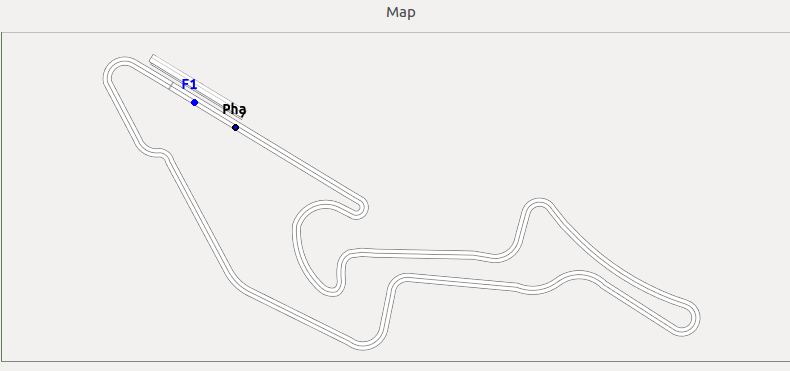
\includegraphics[width=0.98\textwidth]{figures/odom_semiestat_chrono.png}
		\caption{Odometría en ejecución con teleoperador}
		\label{fig.oet}
		\end{center}
\end{figure}

\subsection{Ejecución en movimiento}
Una vez conseguido un algoritmo que procese las imágenes en movimiento con el teleoperador, el alumno puede pasar a la última fase del desarrollo de la solución, el control de movimiento del robot. Para ello deberá utilizar el procesamiento de la imagen realizado en la primera parte del desarrollo del algoritmo para poder dotar al robot de un movimiento en función del filtrado que realice de la línea roja del circuito.
En este punto hay que tener especial cuidado con las curvas dado que la línea varía bruscamente y, con una velocidad elevada, la línea puede salirse del rango de captura de imagen de la cámara y, por lo tanto, el algoritmo producirá un error (a menos que se programe una solución para ese caso). Es por esto que el alumno debe ser consciente de la velocidad de refresco de la imagen de la cámara, 20 frames por segundo, y de la velocidad con la que el nodo recoge las imágenes de la cámara. Esta última función es la más limitante en cuanto a refresco en el procesamiento de la imagen, dado que, aunque utiliza una hebra para la interconexión entre los sensores y actuadores con el nodo académico. Debido a la odometría y a la sincronización, el hilo de ejecución no recoge las 20 imágenes por segundo que capta la cámara sino que dependerá de la potencia computacional de cada ordenador.

\begin{figure}[H]
  \begin{center}
    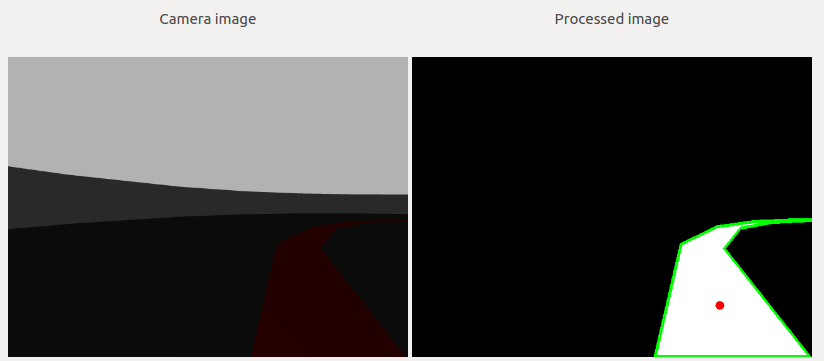
\includegraphics[width=0.98\textwidth]{figures/filtrado_curvas_chrono.png}
		\caption{Ejemplo de procesamiento de la imagen en las curvas}
		\label{fig.pdiecch}
		\end{center}
\end{figure}

Por último, una vez que se ha desarrollado el algoritmo completo, se puede ejecutar la práctica con el algoritmo.

\begin{figure}[H]
  \begin{center}
    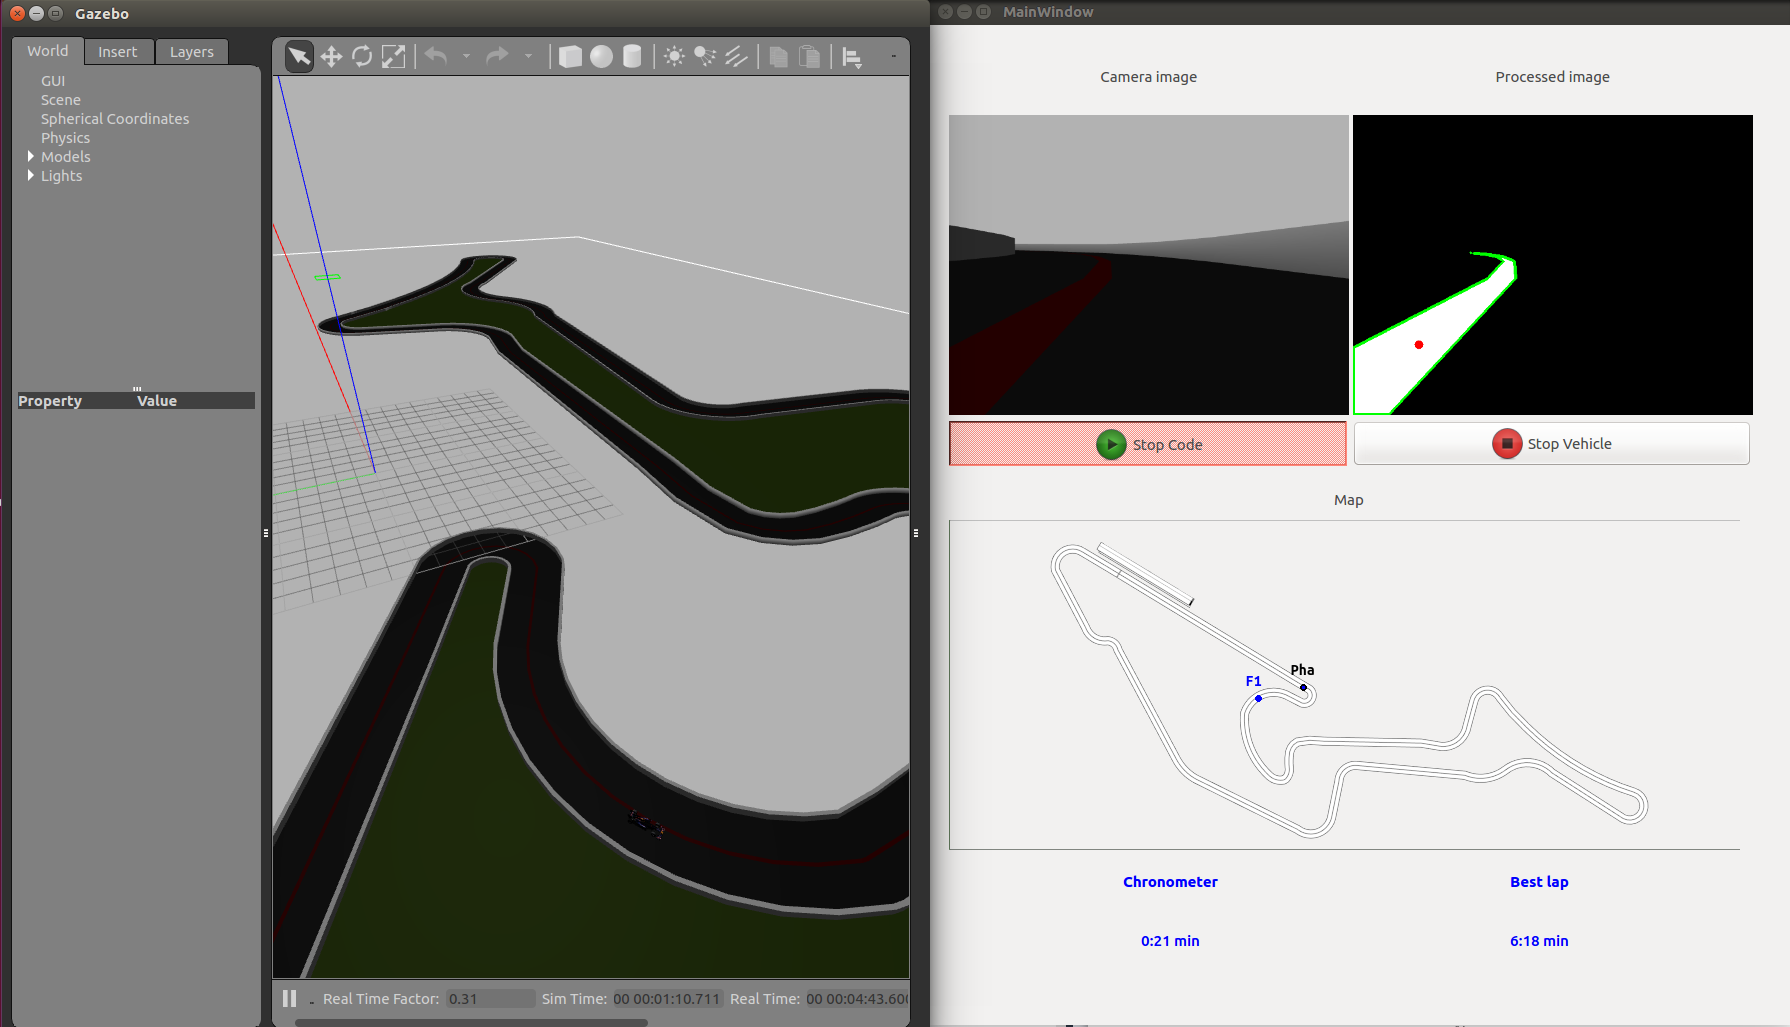
\includegraphics[width=0.98\textwidth]{figures/ejec_algoritmo_ch.png}
		\caption{Ejecución con la solución}
		\label{fig.ealgch}
		\end{center}
\end{figure}

\section{Cuadernillo académico Jupyter}
Como parte paralela a la práctica incluida en \textit{JdeRobot-Academy}, se ha desarrollado la misma práctica en con cuadernillos de \textit{Jupyter}. Gracias a esto, el alumno puede programar y ejecutar el código mediante la utilización del navegador web que prefiera.

Esto supone un paso importante hacia la multiplataforma del entorno docente \textit{JdeRobot Academy}, dado que el alumno puede acceder a las prácticas desde el sistema operativo que prefiera, pues sólo necesita acceso a internet.

Para que sea posible este hecho, ha sido necesaria una reestructuración del nodo académico y de los ficheros que lo componen, además del método de desarrollo del algoritmo.

En primer lugar. el nodo académico tiene la siguiente estructura:

\begin{figure}[H]
  \begin{center}
    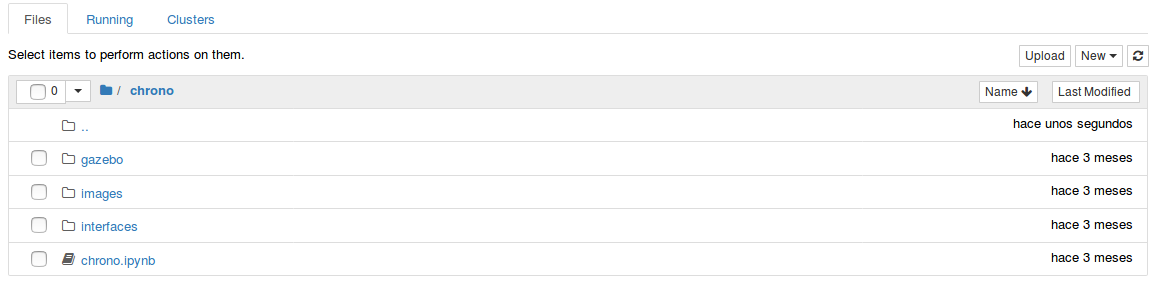
\includegraphics[width=0.98\textwidth]{figures/estructura_jupyter.png}
		\caption{Estructura de la práctica en Jupyter}
		\label{fig.ejch}
		\end{center}
\end{figure}

Como puede verse es diferente a la estructura presente en \textit{JdeRobot-Academy}. Ahora se divide en los siguiente fichero y carpetas:

\begin{itemize}
    \item images: en este directorio aparecen las imágenes contenidas en el cuadernillo.
    \item gazebo: en este directorio está el fichero de configuración con el escenario y con los \textit{drivers} de \textit{ROS-Kinetic}.
    \item interfaces: en este directorio se encuentran los \textit{drivers} de \textit{ROS-Kinetic}.
    \item chrono.ipynb: este fichero es el cuadernillo ejecutable en Jupyter.
\end{itemize}

Para acceder a la práctica, el alumno debe iniciar Jupyter introduciendo en la terminal el siguiente comando:

\lstset{language=bash, breaklines=true, basicstyle=\footnotesize}
\begin{lstlisting}[frame=single]
cd ~/Jupyter
jupyter-notebook
\end{lstlisting}

Con esto se abrirá el navegador web por defecto en la carpeta local Jupyter. Una vez hecho esto, navegaremos hacia el directorio de la práctica de Jupyter ``Chrono'' y abriremos el fichero ``Chrono.ipynb''. Tras esto se mostrará la siguiente imagen del cuadernillo:

\begin{figure}[H]
  \begin{center}
    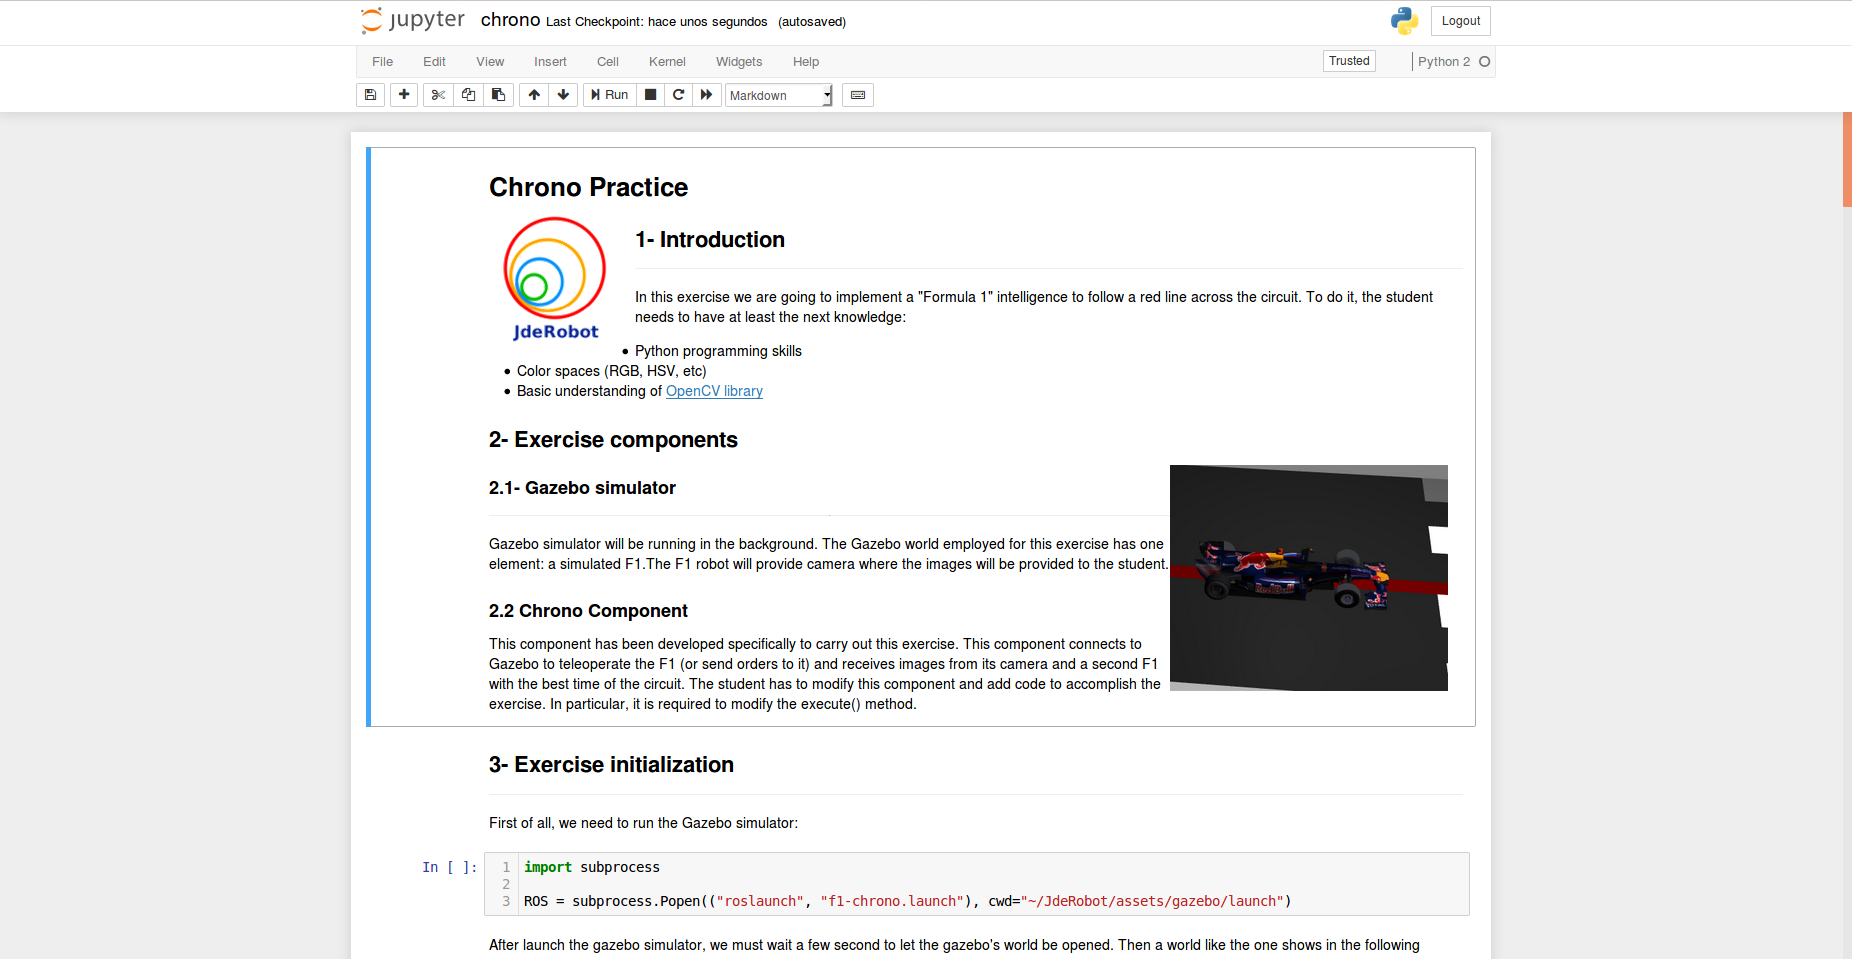
\includegraphics[width=0.98\textwidth]{figures/ipynb_chrono.png}
		\caption{Fichero Chrono.ipynb}
		\label{fig.fcipynb}
		\end{center}
\end{figure}

El alumno deberá ejecutar las celdas con código y seguir el guión mostrado. En primer lugar deberá ejecutar el fichero de configuración del mundo:

\begin{figure}[H]
  \begin{center}
    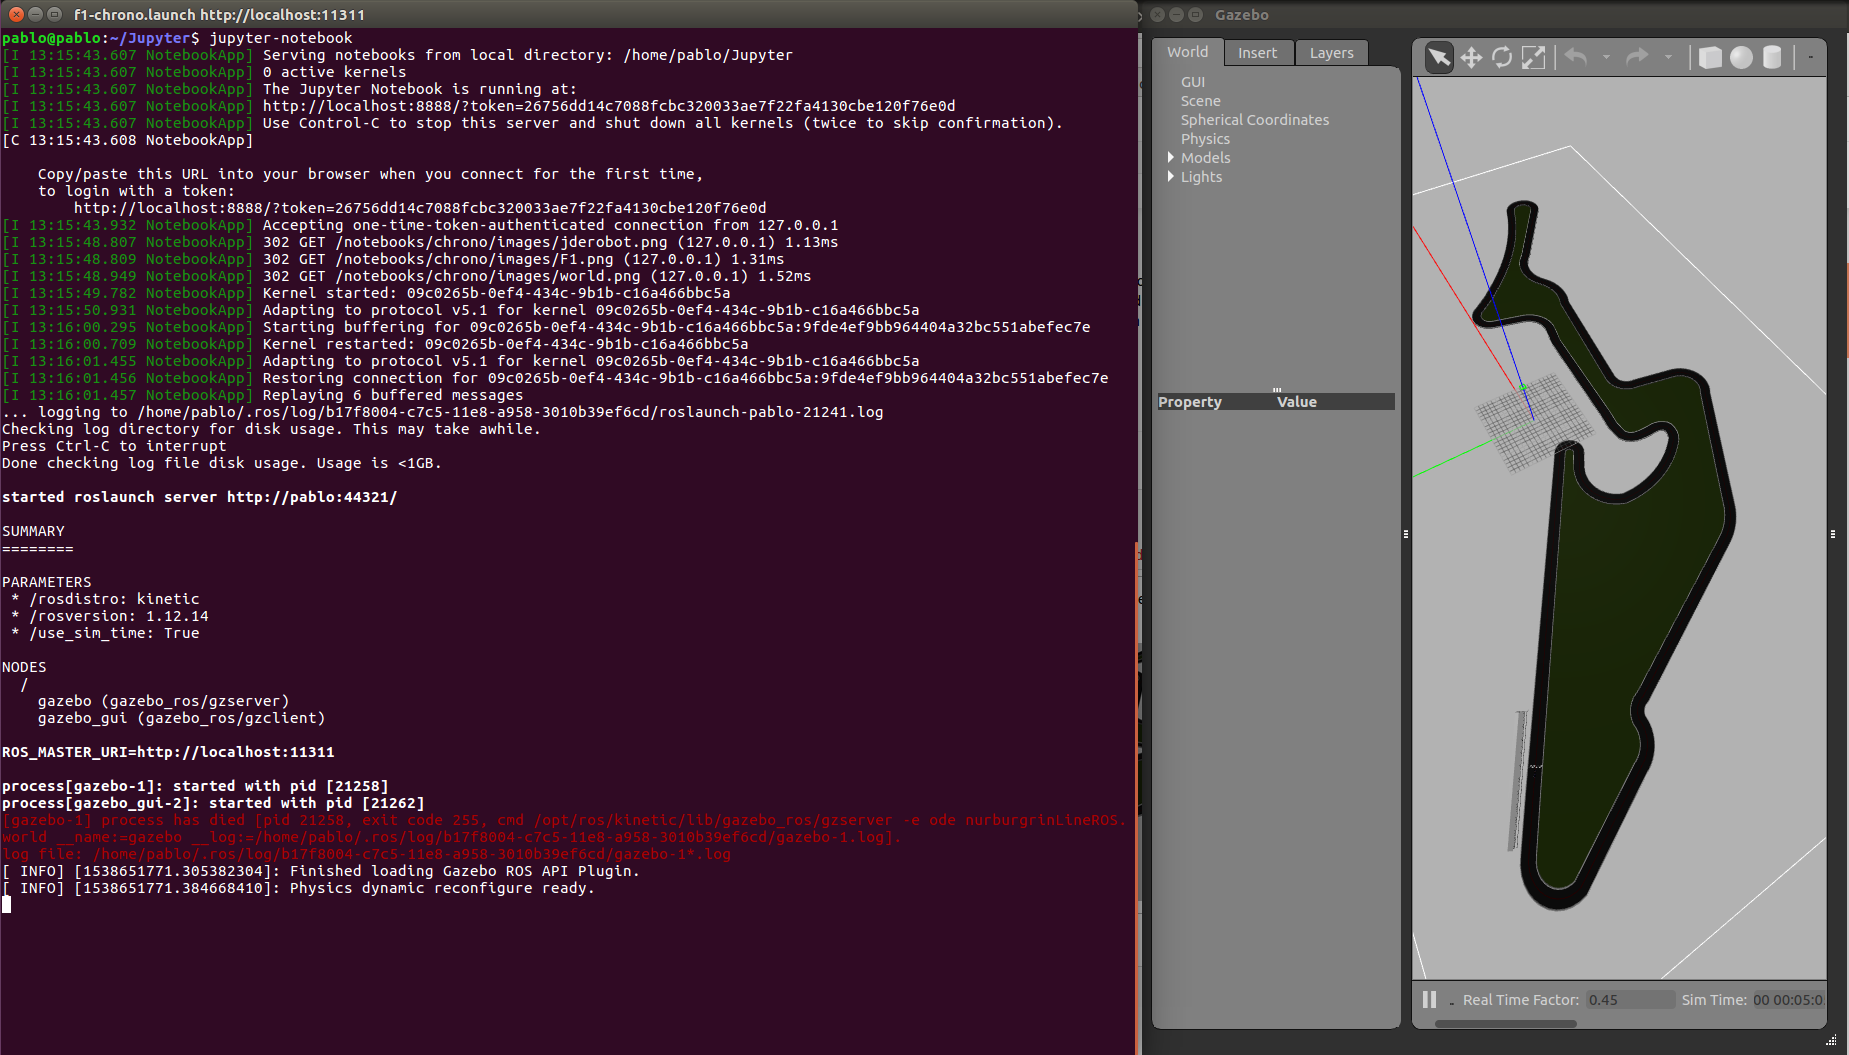
\includegraphics[width=0.98\textwidth]{figures/celda_mundo_chrono.png}
		\caption{Celda con la inicialización del mundo y los drivers}
		\label{fig.cmdc}
		\end{center}
\end{figure}

Cuando se haya abierto el simulador,es necesario importar el módulo del paquete ``MyAlgorithm.py'' y ``Chrono.py'' para tener la funcionalidad proveída en el nodo académico. Para ello, se ejecutará la siguiente celda con el nodo académico de la práctica:

\begin{figure}[H]
    \centering
	\begin{minipage}[h]{.48\linewidth}
    \centering
    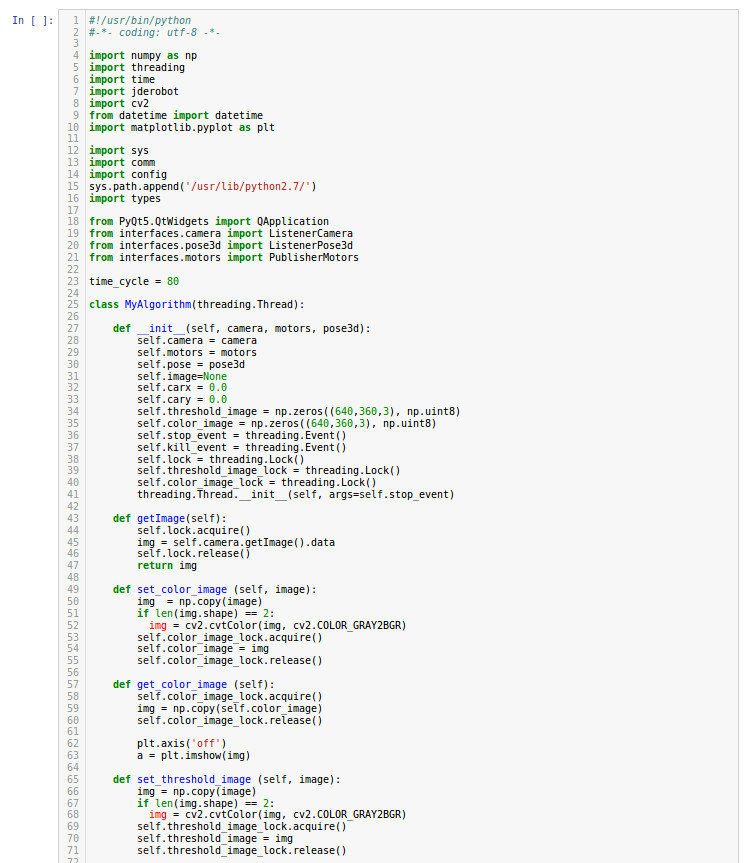
\includegraphics[width=0.98\textwidth]{figures/celda_nodo_chrono1.png}
	 \end{minipage}
    \begin{minipage}[h]{.48\linewidth}
    \centering
    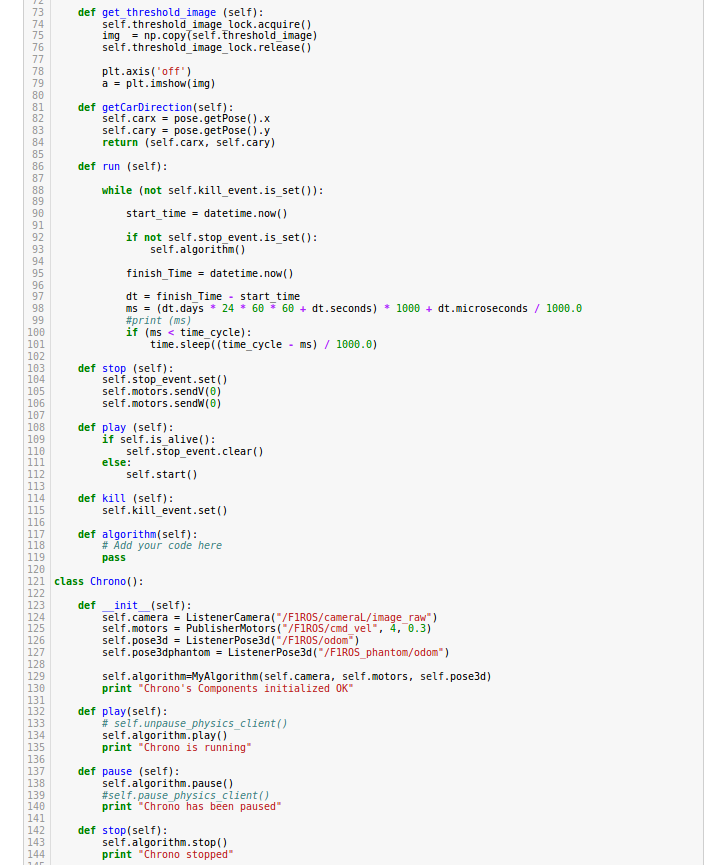
\includegraphics[width=0.98\linewidth]{figures/celda_nodo_chrono2.png}
	\end{minipage}
    \begin{minipage}[h]{.48\linewidth}
    \centering
    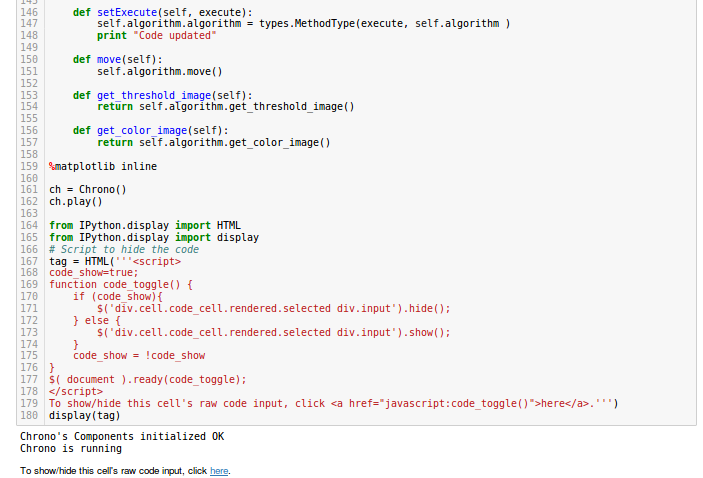
\includegraphics[width=0.98\linewidth]{figures/celda_nodo_chrono3.png}
	\end{minipage}
    \caption{Celda para importar el nodo académico}
		\label{fig.cnach}
\end{figure}


Cuando la ejecución imprima el mensaje ``OK''. El alumno puede comenzar a programar su código en la celda especificada para ello.

\begin{figure}[H]
  \begin{center}
    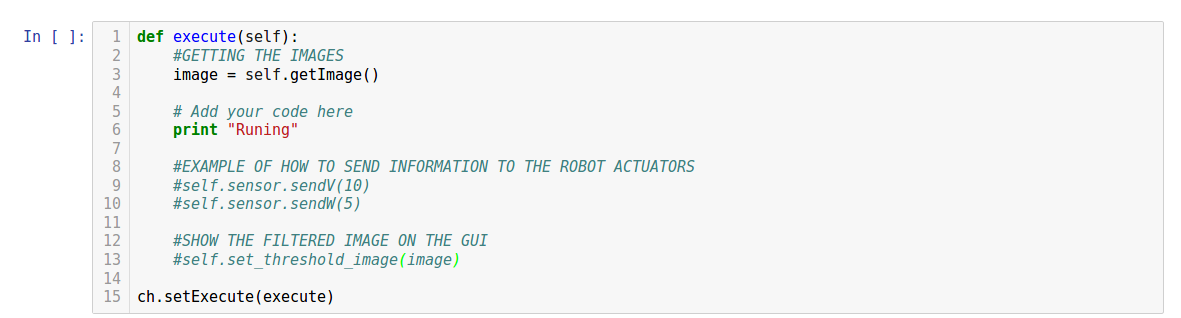
\includegraphics[width=0.98\textwidth]{figures/celda_solucion_chrono.png}
		\caption{Celda con el algoritmo del alumno}
		\label{fig.ccach}
		\end{center}
\end{figure}

Para comprobar el código desarrollado, basta con ejecutar la celda donde ha programado el algoritmo. Si quiere parar la ejecución, es suficiente con pulsar el botón con el icono de ``Stop'' del cuadernillo.

\begin{figure}[H]
    \centering
	\begin{minipage}[h]{.48\linewidth}
    \centering
    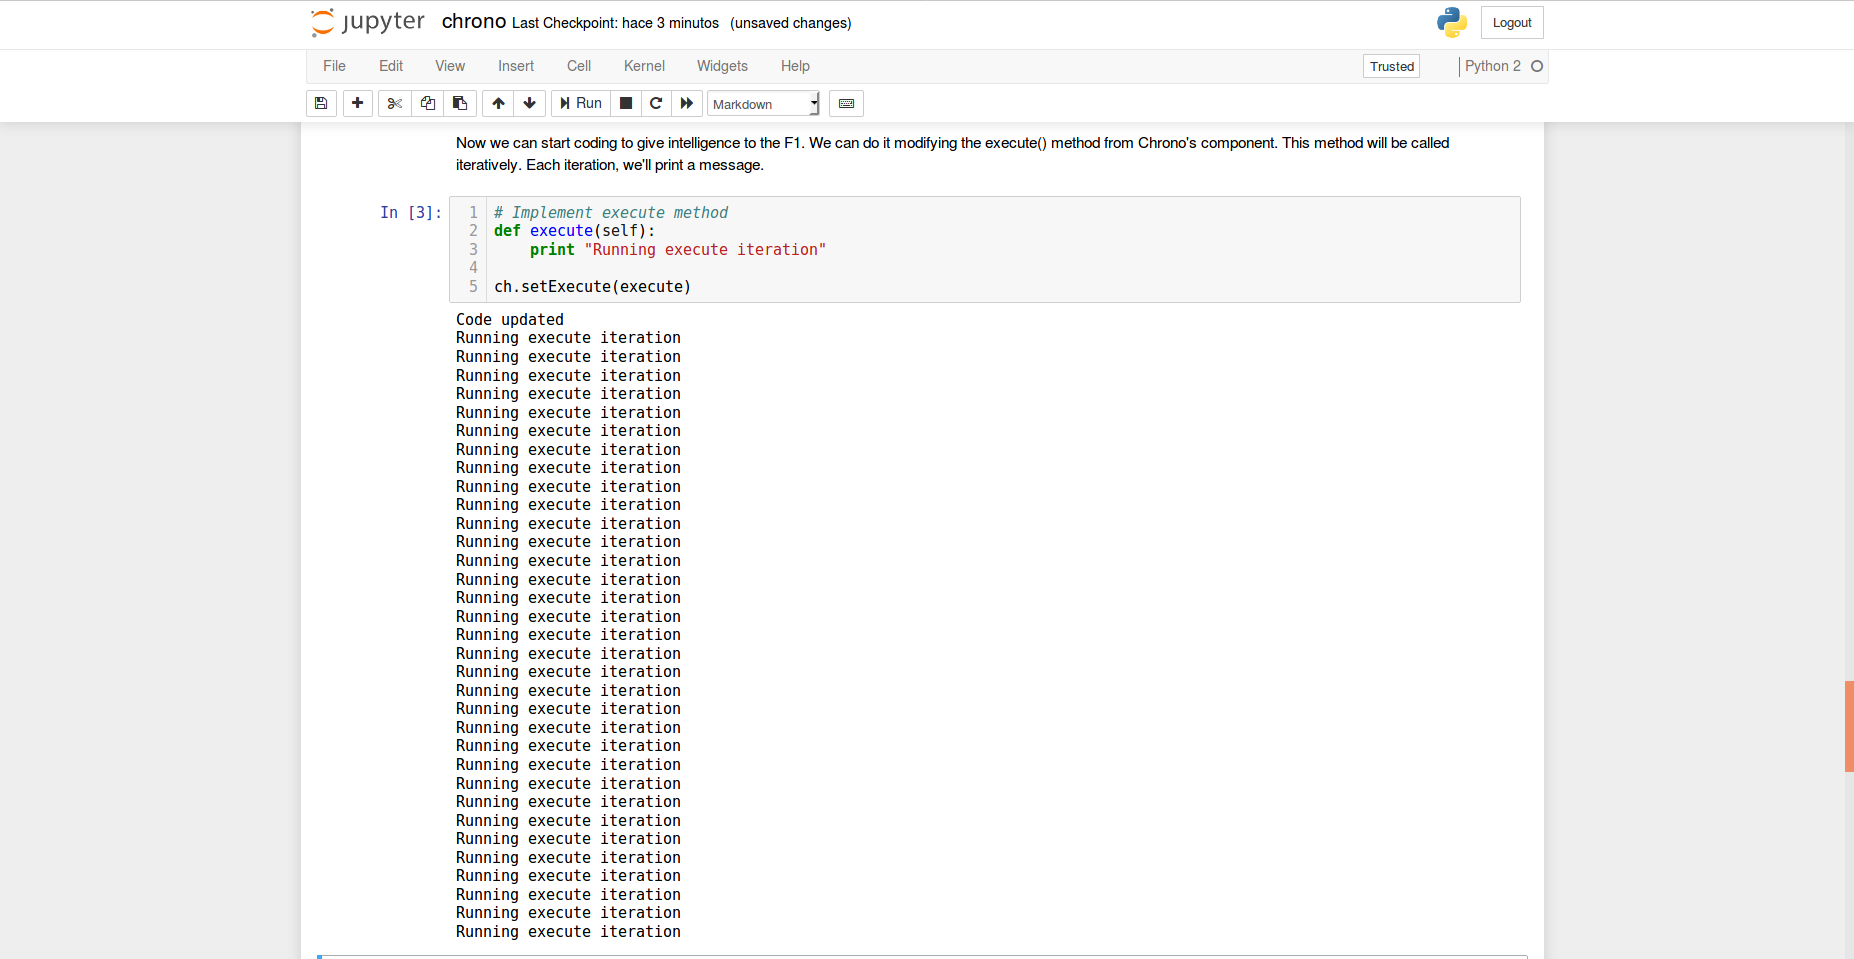
\includegraphics[width=0.98\textwidth]{figures/ejecucion_chrono_jupyter.png}
		\caption{Ejecución de la celda del algoritmo}
		\label{fig.ecj}
	 \end{minipage}
    \begin{minipage}[h]{.48\linewidth}
    \centering
    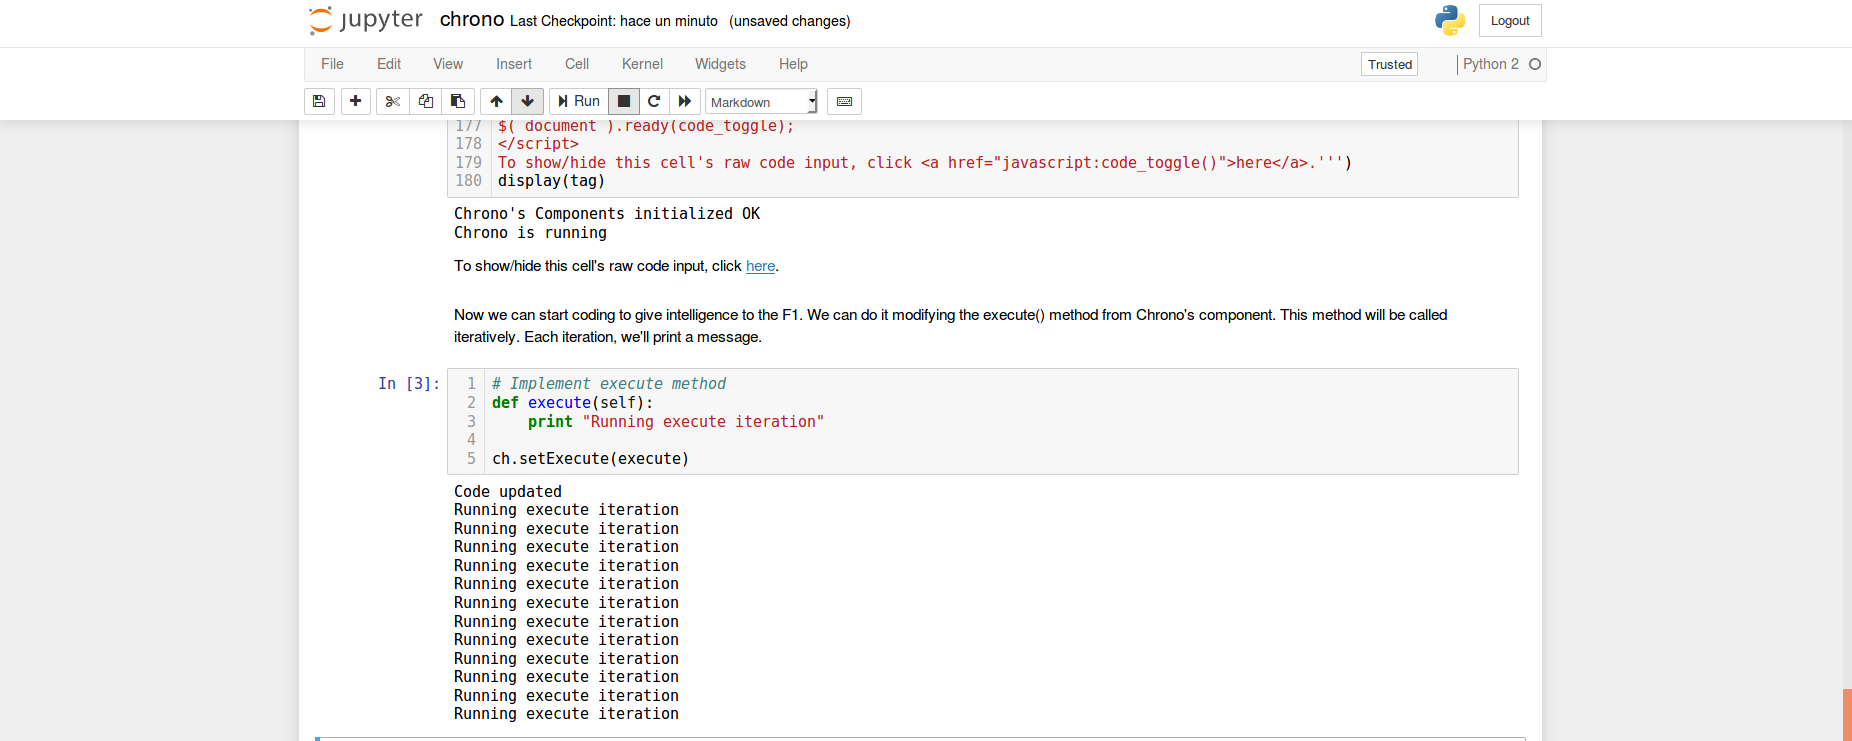
\includegraphics[width=0.98\linewidth]{figures/stop_chrono_jupyter.png}
		\captionof{figure}{Pausa de la ejecución del algoritmo}
		\label{fig:scj}
	\end{minipage}
\end{figure}

Puedes ver un vídeo de la ejecución de Jupyter con esta práctica.\footnote{\url{https://www.youtube.com/watch?v=vTAekepTRkQ}}